\documentclass[11pt, oneside]{scrbook}
\usepackage[sexy]{evan}
\usepackage{esint}
\usepackage{empheq}

\usepackage{calligra}
\DeclareMathAlphabet{\mathcalligra}{T1}{calligra}{m}{n}
\DeclareFontShape{T1}{calligra}{m}{n}{<->s*[2.2]callig15}{}

\newcommand{\scripty}[1]{\ensuremath{\mathcalligra{#1}}}
\newcommand{\scr}{\scripty{r}}

\newcommand{\prob}[1]{\noindent\boxed{\textbf{\sffamily Problem #1}}}

\begin{document}

\title{Electrodynamics Notes}
\subtitle{Phillips Academy Andover\\
PRO601 Physics IP: Advanced Electrodynamics with Jeffrey Shi\\
Mentored by Fei Yao}
\author{William Yue}
\date{Spring 2022, v.$\alpha$.20220421}
\maketitle

\chapter*{Introduction}

This document contains my notes for my Spring Term Physics IP (Independent Project) entitled \textit{Advanced Electrodynamics}, taken during my last term at Phillips Academy Andover. Jeffrey Shi was my partner for the group IP and our mentor was Ms.~Fei Yao. Our main reference text is \textit{Introduction to Electrodynamics}, 4th edition by Griffiths.

% I have also included some of our solutions to selected problems from the text. The numbering of these problems follows the book, rather than this document. We tried to tackle every problem marked with a bullet $\bullet$ or an exclamation point \textbf{!}. We also tackled any other problems that we found interesting.

\tableofcontents

\chapter{Vector Analysis}

\section{Vector Algebra}

\subsection{Vector Operations}

\subsection{Vector Algebra: Component Form}

These first two subsections reviews the basics of vectors; for the purpose of these notes, I will assume the reader already has a strong basic understanding of vectors, so they will be left empty.

\subsection{Triple Products}

The output of a cross product $\vec{b}\times\vec{c}$ is a vector, so it can be dotted or crossed with another vector $\vec{a}$ to form a triple product.

The \vocab{scalar triple product} $\vec{a}\cdot(\vec{b}\times\vec{c})$ gives the signed volume of the parallelepiped generated by $\vec{a},\vec{b},\vec{c}$. Therefore,
\begin{claim}
$\vec{a}\cdot(\vec{b}\times\vec{c})=\vec{b}\cdot(\vec{c}\times\vec{a})=\vec{c}\cdot(\vec{a}\times\vec{b})$.
\end{claim}
Notice that we preserved the cyclic order of the vectors in this case; if we flip the order (e.g. $\vec{a}\cdot(\vec{c}\times\vec{b})$), then we obtain the same value with opposite sign. In component form, we have
\[\vec{a}\cdot(\vec{b}\times\vec{c})=\det\begin{bmatrix}
a_x & a_y & a_z\\
b_x & b_y & b_z\\
c_x & c_y & c_z
\end{bmatrix},\]

The \vocab{vector triple product} $\vec{a}\times (\vec{b}\times \vec{c})$ can be simplified by the so-called ``$bac-cab$ rule":
\begin{claim}
$\vec{a}\times(\vec{b}\times\vec{c})=\vec{b}(\vec{a}\cdot\vec{c})-\vec{c}(\vec{a}\cdot\vec{b}).$
\end{claim}
Note that cross-products are not associative, so the order of parentheses matters. By repeated application of this fact, it is never necessary for an expression to contain more than one cross product in any term. For example,
\[(\vec{a}\times \vec{b})\cdot(\vec{c}\times\vec{d})=(\vec{b}\times(\vec{c}\times \vec{d}))\cdot \vec{a}=(\vec{c}(\vec{b}\cdot\vec{d})-\vec{d}(\vec{b}\cdot\vec{c}))\cdot\vec{a}=(\vec{a}\cdot\vec{c})(\vec{b}\cdot\vec{d})-(\vec{a}\cdot\vec{d})(\vec{b}\cdot\vec{c}),\]
where in the first equality we utilized the scalar triple product identity $\vec{a}\cdot(\vec{b}\times\vec{c})=\vec{b}\cdot(\vec{c}\times\vec{a})$.

\subsection{Position, Displacement, and Separation Vectors}

\begin{definition}
Given a coordinate system with origin $\mathcal{O}$, the vector from $\mathcal{O}$ to some point is the \vocab{position vector}
\[\vec{r}:=x\hat{x}+y\hat{y}+z\hat{z},\]
where $(x,y,z)$ are the Cartesian coordinates of the point. 
\end{definition}
Note that the distance from the point to the origin is
\[r=|\vec{r}|=\sqrt{x^2+y^2+z^2}\]
and the unit vector in the direction of $\vec{r}$ is 
\[\hat{r}=\frac{\vec{r}}{r}=\frac{x\hat{x}+y\hat{y}+\hat{z}}{\sqrt{x^2+y^2+z^2}}.\]

\begin{definition}
The \vocab{infinitesimal displacement vector} from $(x,y,z)$ to $(x+dx,y+dy,z+dz)$ is denoted by
\[d\vec{\ell}=dx\hat{x}+dy\hat{y}+dz\hat{z}.\]
\end{definition}
Oftentimes in electrodynamics, we encounter problems involving two points:
\begin{itemize}
    \item A \vocab{source point} $\vec{r'}$, where an electric charge is located,
    \item A \vocab{field point} $\vec{r}$, where we are calculating the electric or magnetic field.
\end{itemize}
In the situation when $\vec{r'}\neq \vec{0}$, it is useful to adopt a shorthand notation for the \vocab{separation vector} from the source point to the field point; we will use the script letter
\[\vec{\scripty{r}}:=\vec{r}-\vec{r'}.\]

\subsection{How Vectors Transform}

What exactly is a vector? You might have learned it as ``a quantity with a magnitude and direction," but this isn't exactly satisfactory...

Perhaps a 3-dimensional vector is simply anything with three real components that combine properly under addition. However, what if we considered some silly example like a barrel with $N_x$ pear, $N_y$ apples, and $N_z$ bananas? Is $\vec{N}=N_x\hat{x}+N_y\hat{y}+N_z\hat{z}$ suddenly a vector? Surely not---what is the direction? What is wrong with it?

The answer is that $\vec{N}$ \textit{doesn't transform properly when you change coordinates}.

In three dimensions, if a $x,y,z$ system is rotated to some $\ol{x},\ol{y},\ol{z}$, system, then the coordinates of some vector $\vec{a}$ undergo a matrix transformation
\[
\begin{bmatrix}
\ol{a}_x\\\ol{a}_y\\\ol{a}_z
\end{bmatrix}=\begin{bmatrix}
R_{xx} & R_{xy} & R_{xz}\\
R_{yx} & R_{yy} & R_{yz}\\
R_{zx} & R_{zy} & R_{zz}
\end{bmatrix}\cdot\begin{bmatrix}
a_x\\a_y\\a_z
\end{bmatrix}\qquad\text{or}\qquad \vec{\ol{a}}=R\vec{a}.,
\]
where $R_{ij}$ are some products of trigonometric functions (or it could simply be any arbitrary linear transformation of $\mathbb{R}^3$). More compactly, we can write it as
\[\ol{a}_i=\sum_{j=1}^3 R_{ij}a_j,\]
where index 1 stands for $x$, etc. 

The components of $\vec{N}$ clearly don't transform in this way.

\begin{definition}
Formally, a \vocab{vector} is any set of three components that transforms in the same manner as a displacement when you change coordinates.
\end{definition}

Therefore, displacement is the \textit{model} for the behavior of all vectors.

\begin{definition}
A \vocab{second-order tesnor} is a quantity with \textit{nine} components: $T_{xx}$, $T_{xy}$, $T_{xz}$, $T_{yx}$,\dots ,$T_{zz}$. These transform with \textit{two} factors of $R$:
\[\ol{T}_{ij}=\sum_{k=1}^3\sum_{\ell=1}^3R_{ik}R_{j\ell}T_{k\ell}.\]
You can also rewrite this in matrix form as $\ol{T}=RTR^T$.
\end{definition}

In general, an $n$th-order tensor has $n$ indices and $3^n$ components (in $\mathbb{R}^3$), and transforms with $n$ factors of $R$. Therefore, a scalar is a tensor of order zero (indeed, note that scalars never change under coordinate changes) and a vector is a tensor of order one.

\section{Differential Calculus}

\subsection{``Ordinary" Derivatives}

Suppose we have a single-variable function $f(x)$. What does the derivative $\frac{df}{dx}$ do?

\begin{moral}
The derivative of a function $df/dx$ tells us how rapidly the function $f$ varies when we change $x$ by a tiny amount $dx$.
\end{moral}

In other words, if $x$ is incremented by an infinitesimal amount $dx$ and $f$ changes by an amount $df$, then the derivative is the proportionality factor:
\[df=\left(\frac{df}{dx}\right)dx.\]
From a geometric perspective, the derivative $\frac{df}{dx}$ gives the \textit{slope} at any point on the graph of $f$ against $x$.

\subsection{Gradient}

That's all well and good for one variable. What about functions of three variables, say temperature $T(x,y,z)$ in $\mathbb{R}^3$? 

How do we generalize the notion of the derivative to functions like $T$? 

We want the derivative to tell us how $T$ changes when we move a tiny distance. However, $T$ may change at a different rate depending on the direction we move in! In a room, nudging $z$ will probably have a much higher affect on the temperature than nudging $x$ or $y$ the same amount.

Fortunately, the situation is not so bad: it turns out that when we zoom in enough, a differentiable function $T$ will always look like a plane, linear in all variables:
\[dT=\left(\frac{\partial T}{\partial x}\right)dx+\left(\frac{\partial T}{\partial y}\right)dy+\left(\frac{\partial T}{\partial z}\right)dz.\]
The proportionality constants are \textit{partial derivatives}, which measure the change in $T$ when you hold all variables constant except for the one in the denominator: therefore, $\frac{\partial T}{\partial x}$ measures the rate of change of $T$ when you move only $x$ by an infinitesimal amount.

This is a rather nice result: we don't need to compute the rate of change of $T$ among all possible directions; three directions $x,y,z$ suffice. 

We can also use it to define another concept. The equation is reminiscent of a dot product:
\[dT=\left(\frac{\partial T}{\partial x}\hat{x}+\frac{\partial T}{\partial y}\hat{y}+\frac{\partial T}{\partial z}\hat{z}\right)\cdot(dx \hat{x}+dy\hat{y}+dz \hat{z}).\]
We give the first vector in this dot product a name:
\begin{definition}
The \vocab{gradient} of a scalar function $T$ is the vector quantity
\[\nabla T:=\frac{\partial T}{\partial x}\hat{x}+\frac{\partial T}{\partial y}\hat{y}+\frac{\partial T}{\partial z}\hat{z}.\]
\end{definition}

Then, $dT=\nabla T\cdot d\vec{\ell}$. Wait... what just happened? This means that if we move by a small vector $d\vec{\ell}$, then the change in $T$ is given by taking the dot product of this small shift vector by the gradient of $T$ at that point. 

Let's dissect this a little more: we can expand the dot product to get
\[dT=\nabla T\cdot d\vec{\ell}=|\nabla T||d\vec{\ell}|\cos\theta,\]
where $\theta$ is the angle between this new gradient vector we just defined and the small shift $d\vec{\ell}$ that we take. Suppose we \textit{fix} the magnitude of $d\vec{\ell}$, so we're always stepping the same tiny amount. Then, if we search various directions by varying $\theta$, notice the \textit{maximum} change in $T$ occurs when $\theta=0$. 

Focusing on this case, we extract the following intuition on what exactly the gradient is:

\begin{moral}
The gradient $\nabla T$ points in the direction of maximum increase of the function $T$. Moreover, its magnitude $|\nabla T|$ gives the rate of increase of $T$ along this maximal direction.
\end{moral}

If we point $d\vec{\ell}$ in the opposite direction of the gradient ($\theta=180^\circ$), then the rate of change is precisely the negative, which makes sense. Also note if we point perpendicular to the gradient ($\theta=90^\circ$), $T$ doesn't change along this direction at all.

Here's a nice picture to keep in your mind: suppose you're on a large, bumpy mountain. We can characterize the surface of this mountain by the \textit{two}-variable function $h(x,y)$ which gives the height of the mountain above any point $(x,y)$ in the plane. Standing at any point $(x,y)$, you can look around and find the direction of steepest ascent---that is the \textit{direction} of the gradient. If you calculate the slope of the mountain in that direction (rise over run)---that is the \textit{magnitude} of the gradient. 

As a person standing on the mountain, if you zoom in enough, you can disregard any large scale bumps in the mountain: it simply looks like a plane; this is what allows the dot product formula $dT=\nabla T\cdot d\vec{\ell}$ to work (with this picture in your mind, reason through the $\theta=180^\circ$ and $\theta=90^\circ$ cases again. This is analogous to the one-variable case, where taking the derivative assumes that when you zoom far in enough on $f$, you get something that looks like a straight line. 

\begin{definition}
We call points where $\nabla T=\vec{0}$ \vocab{stationary points}.
\end{definition}

These can be maximums (summits), minimums (valleys), saddle points (a pass), or ``shoulders."

% \subsubsection*{Problems}

% \prob{1.13} Let $\vec{\scripty{r}}$ be the separation vector from a fixed point $(x',y',z')$ to the point $(x,y,z)$, and let $\scripty{r}$ be its length. Show that
% \begin{enumerate}[(a)]
%     \item $\nabla(\scr^2)=2\vec{\scr}$.
%     \item $\nabla(1/\scr)=-\hat{\scr}/\scr^2$.
%     \item What is the \textit{general} formula for $\nabla(\scr^n)$?
% \end{enumerate}

% \begin{proof}
% We skip to part (c), as (a) and (b) are simply special cases $n=2$ and $n=-1$, respectively. First, note that $\vec{\scr}=(x-x')\hat{x}+(y-y')\hat{y}+(z-z')\hat{z}$. Now,
% \[\nabla(\scr^n)=\frac{\partial \scr^n}{\partial x}\hat{x}+\frac{\partial \scr^n}{\partial y}\hat{y}+\frac{\partial \scr^n}{\partial z}\hat{z}=\sum \frac{\partial \scr^n}{\partial x}\hat{x},\]
% where the sum is over $x,y,z$. Now, note that
% \[\frac{\partial \scr^n}{\partial x}=n\scr^{n-1}\cdot\frac{\partial \scr}{\partial x}.\]
% Noting that $\scr=\sqrt{(x-x')^2+(y-y')^2+(z-z')^2}$, we have that
% \[\frac{\partial\scr}{\partial x}=\frac{1}{2}\cdot \frac{1}{\scr}\cdot (2x-2x')=\frac{x-x'}{\scr}.\]
% Therefore,
% \[\nabla(\scr^n)=n\scr^{n-1}\cdot \sum \frac{(x-x')\hat{x}}{\scr}=n\scr^{n-1}\cdot\frac{\vec{\scr}}{\scr}=\boxed{n\scr^{n-1}\hat{\scr}}.\]
% \end{proof}

% TODO: insert 1.13

\subsection{The Del Operator}

\begin{definition}
We define the $\vocab{del operator}$ as the vector operator
\[\nabla:=\hat{x}\frac{\partial}{\partial x}+\hat{y}\frac{\partial}{\partial y}+\hat{z}\frac{\partial}{\partial z}.\]
\end{definition}

The del operator $\nabla$ is not really a vector; it's more of an instruction. When given a scalar function $T$ to act upon, it produces the gradient $\nabla T$.

Nonetheless, $\nabla$ can mimic the behavior of an ordinary vector in virtually every way, if we translate ``multiply" as ``act upon." It is great notational simplification, even if it's a bit of an abuse. Indeed, we can mimic all three types of vector products:

\begin{enumerate}
    \item On a scalar function $T$, $\nabla$ can act to give the gradient $\nabla T$;
    \item On a vector function $\vec{v}$, via the dot product, to give the \vocab{divergence} $\nabla\cdot \vec{v}$;
    \item On a vector function $\vec{v}$, via the cross product, to give the \vocab{curl} $\nabla\times \vec{v}$.
\end{enumerate}
The following sections will analyze the divergence and curl.

\subsection{The Divergence}

\begin{definition}
The \vocab{divergence} of a vector function $\vec{v}$ is the scalar quantity
\[\nabla\cdot \vec{v}=\frac{\partial v_x}{\partial x}+\frac{\partial v_y}{\partial y}+\frac{\partial v_z}{\partial z}.\]
\end{definition}

The name \textit{divergence} is well-chosen: $\nabla\cdot\vec{v}$ is a measure of how much the vector field $\vec{v}$ spreads out (i.e. diverges) from a given point. 

Imagined a lake with streams and eddies where $\vec{v}$ represented the velocity of the water at any given point. If you drop some particles into the lake at any given point, if they spread out, that's a point of positive divergence, while if they collect together, that's a point of negative divergence. The points of positive divergence are sources, while the points of negative divergence are sinks. (This analogy is not perfect, since water is generally incompressible, i.e. has zero divergence; however, you can imagine there are literal underwater faucets or drains adding or removing water from certain places.) 

\begin{moral}
The divergence of a vector field $\vec{v}$ measures how much the vectors ``spread out" or ``collect in" at any given point.
\end{moral}

% TODO: maybe add in some pictures

\subsection{The Curl}

\begin{definition}
The \vocab{curl} of a vector function $\vec{v}$ is the vector quantity
\begin{align*}
    \nabla\times\vec{v}&=\det\begin{bmatrix}
    \hat{x} & \hat{y} & \hat{z}\\
    \partial/\partial x & \partial/\partial y & \partial/\partial z\\
    v_x & v_y & v_z
    \end{bmatrix}\\
    &=\left(\frac{\partial v_z}{\partial y}-\frac{\partial v_y}{\partial z}\right)\hat{x}+\left(\frac{\partial v_x}{\partial z}-\frac{\partial v_z}{\partial x}\right)\hat{y}+\left(\frac{\partial v_y}{\partial x}-\frac{\partial v_x}{\partial y}\right)\hat{z}.
\end{align*}
\end{definition}

The name \textit{curl} is also well-chosen: $\nabla \times \vec{v}$ measures how much the vector field $\vec{v}$ rotates (i.e. curls) around a given point. The direction of the vector $\nabla\times\vec{v}$ is given by the right hand rule: if you curl your fingers in the same direction as the vectors are curling, your thumb points in the direction of $\nabla\times\vec{v}$.

In the lake analogy, if you drop a toothpick, if it starts to rotate, then there is nonzero curl at that point. If it rotates counterclockwise, the curl points upward (positive $z$), while if it rotates clockwise, the curl points downward (negative $z$).

\begin{moral}
The curl of a vector field $\vec{v}$ measure how much the vectors ``swirl" around any given point, and also give the direction of this rotation by the right hand rule.
\end{moral}

\subsection{Product Rules}

The vector derivatives of sums and scalar products are rather simple; 
they're just what you would expect.

\begin{proposition}[Vector derivative sum rules]
    We have that
    \begin{itemize}
        \item $\nabla(f+g)=\nabla f+\nabla g$,
        \item $\nabla\cdot(\vec{a}+\vec{b})=(\nabla\cdot \vec{a}) + (\nabla \cdot \vec{b})$,
        \item $\nabla\times(\vec{a}+\vec{b})=(\nabla\times \vec{a}) + (\nabla \times \vec{b})$.
    \end{itemize}
\end{proposition}

\begin{proposition}[Vector derivative scalar multiplication rules]
    We have that
    \begin{itemize}
        \item $\nabla(kf)=k\nabla f$,
        \item $\nabla\cdot(k\vec{a})=k(\nabla\cdot\vec{a})$,
        \item $\nabla\times(k\vec{a})=k(\nabla\times\vec{a})$.
    \end{itemize}
\end{proposition}

The product rules, however, are not so simple.
There are two ways to construct a scalar function as a product of two functions:
either by multiplying to scalar functions to get $fg$
or by taking the dot product of two vector functions to get $\vec{a}\cdot\vec{b}$.
In addition, there are two ways to construct a vector function as a product of two functions:
either by multiplying a scalar function by a vector function to get $f\vec{a}$,
or by taking the cross product of two vector functions to get $\vec{a}\times\vec{b}$.

You can take the gradient of the two products that output a scalar function,
as well as the divergence or curl of the two products that output a vector function,
resulting in \textit{six} product rules.

In general, product rules involving a scalar function are easy, and exactly what you expect (in the divergence/curl formulas, the $\nabla$ on the scalar function turns into a gradient). The product rules involving dot and cross products of two vector functions are more complicated, however.

\begin{proposition}[Gradient product rules]
    We have that
    \begin{itemize}
        \item $\nabla(fg)=f\nabla g+g\nabla f$,
        \item $\nabla(\vec{a}\cdot\vec{b}) = \vec{a}\times(\nabla\times \vec{b}) + \vec{b}\times(\nabla\times \vec{a})+(\vec{a}\cdot\nabla)\vec{b}+(\vec{b}\cdot\nabla)\vec{a}$.
    \end{itemize}
\end{proposition}

\begin{proposition}[Divergence product rules]\label{divprodrul}
    We have that
    \begin{itemize}
        \item $\nabla\cdot(f\vec{a})=f(\nabla\cdot\vec{a})+\vec{a}\cdot(\nabla f)$,
        \item $\nabla\cdot(\vec{a}\times\vec{b})=\vec{b}\cdot(\nabla\times\vec{a})-\vec{a}\cdot(\nabla\times\vec{b})$.
    \end{itemize}
\end{proposition}

\begin{proposition}[Curl product rules]
    We have that
    \begin{itemize}
        \item $\nabla\times(f\vec{a})=f(\nabla\times\vec{a})+\vec{a}\cdot(\nabla f)$,
        \item $\nabla\times(\vec{a}\times\vec{b})=(\vec{b}\cdot \nabla)\vec{a}-(\vec{a}\cdot\nabla)\vec{b}+\vec{a}(\nabla\cdot\vec{b})-\vec{b}(\nabla\cdot\vec{a})$.
    \end{itemize}
\end{proposition}

\subsection{Second Derivatives}

We have covered the three possible first derivatives using the del operator. By using the del operator twice, we can construct \textit{five} species of second derivatives.

Since the gradient and curl are vector, we can take the divergence or curl of them. Since the divergence is a scalar, we can only take the gradient of it. Let's consider these possibilities:

\begin{definition}
    We call the divergence of the gradient of a scalar function $T$ the \vocab{Laplacian} of $T$, denoted $\nabla^2T$. It is equal to
    \begin{align*}
    \nabla\cdot(\nabla T)&=\left(\hat{x}\frac{\partial}{\partial x}+\hat{y}\frac{\partial}{\partial y}+\hat{z}\frac{\partial}{\partial z}\right)\cdot\left(\hat{x}\frac{\partial T}{\partial x}+\hat{y}\frac{\partial T}{\partial y}+\hat{z}\frac{\partial T}{\partial z}\right)\\
    &=\frac{\partial^2T}{\partial x^2}+\frac{\partial^2T}{\partial y^2}+\frac{\partial^2T}{\partial z^2}.
    \end{align*}
\end{definition}

\begin{definition}
    We can also refer to the \vocab{Laplacian} of a vector function, which is simply defined as
    \[\nabla^2\vec{v}:=(\nabla^2 v_x)\hat{x}+(\nabla^2 v_y)\hat{y}+(\nabla^2 v_z)\hat{z}.\]
\end{definition}
The \textit{curl} of the gradient, however, is always equal to zero:
\[\nabla\times(\nabla T)=\vec{0}.\]
A proof of this by components amounts to the fact that $\frac{\partial^2T}{\partial x\partial y}=\frac{\partial^2T}{\partial y\partial x}$.

\begin{remark}\label{remarkcurlgrad}
There is a simple physical explanation for why the curl of the gradient always vanishes. Imagine $T$ represents the height of some mountain; the gradient tells you which direction walks you upwards. If there was nonzero curl of the gradient, this would amount to the gradient vector going around in a closed loop; however, this would mean there is a closed loop where you're always travelling upwards, which is impossible! You can't end up in the same place but be at a higher height.

In essence, we're combining the fundamental theorems of gradients and curls, which will be introduced in the next section. By the fundamental theorem of curl (Stokes' Theorem), the surface integral of the curl of the gradient of $T$ is equal to the line integral of the gradient of $T$ around the boundary of that surface. Then, the fundamental theorem of gradient implies that this loop integral equals 0. In symbols,
\[\iint_\mathcal{S}\nabla\times(\nabla T)\cdot d\vec{a}=\oint_{\partial \mathcal{S}}\nabla T\cdot d\vec{\ell}=\vec{0}\]
since $\partial^2\mathcal{S}=0$.
\end{remark}

Like the curl of the gradient, the \textit{divergence} of the curl is always equal to zero:
\[\nabla\cdot(\nabla\times \vec{v})=0.\]
This can also be easily checked through the definitions of divergence and curl.

\begin{remark}\label{remarkdivcurl}
There is also an explanation of why this is true by combining the fundamental theorems of divergences and curls (also introduced in the next section). By the fundamental theorem of divergence (Gauss's Theorem), the volume integral of the divergence of the curl of $\vec{v}$ is equal to the surface integral of the curl of $\vec{v}$ over the boundary of the volume. Then, the fundamental theorem of curl (Stokes' Theorem) implies that this closed surface integral equals 0. In symbols,
\[\iiint_\mathcal{V}\nabla\cdot(\nabla\times \vec{v}) d\tau=\oiint_{\partial\mathcal{V}}(\nabla\times\vec{v})\cdot d\vec{a}=\oint_{\partial^2\mathcal{V}}\vec{v}\cdot d\vec{\ell}=0\]
since $\partial^2\mathcal{V}=0$.
\end{remark}

\begin{remark}
Remarks \ref{remarkcurlgrad} and \ref{remarkdivcurl} both rely on the fact that the boundary operator $\partial$ satisfies $\partial^2=0$: the first uses the fact that the boundary of the boundary of a surface (the boundary of a closed loop) is nothing, and the second uses the fact that the boundary of the boundary of a volume (the boundary of a closed surface) is nothing.
\end{remark}

\begin{definition}
    We simply refer to $\nabla(\nabla\cdot \vec{v})$ as the \vocab{gradient of the divergence} of $\vec{v}$. Note that this is \textit{not} equal to the Laplacian.
\end{definition}

This quantity seldom appears in physics, so we don't give it a special name. The curl of the curl is also nothing new:

\begin{definition}
    We also simply refer to $\nabla\times(\nabla \times \vec{v})$ as the \vocab{curl of the curl} of $\vec{v}$.
\end{definition}

It turns out that
\[\nabla\times(\nabla\times \vec{v})=\nabla(\nabla\times \vec{v})-\nabla^2\vec{v}.\]
Often, this is actually used to \textit{define} the Laplacian of a vector function $\nabla^2\vec{v}$, since our previous definition relied on Cartesian coordinates $\hat{x}, \hat{y}, \hat{z}$, which is undesirable.

\section{Integral Calculus}

\subsection{Line, Surface, and Volume Integrals}

\begin{definition}
    A \vocab{line integral} is an expression of the form 
    \[\int_{\vec{a}}^{\vec{b}}\vec{v}\cdot d\vec{\ell},\]
    where $\vec{v}$ is some vector function and $d\vec{\ell}$ is the infinitesimal displacement vector.
    These two vectors are dotted along every point on some prescriped path $\mathcal{P}$ from point $\vec{a}$ to point $\vec{b}$;
    these values are summed by the integral to obtain the result.

    If $\mathcal{P}$ is a closed loop, i.e. $\vec{a}=\vec{b}$, then we instead write a loop integral
    \[\oint\vec{v}\cdot d\vec{\ell}.\]
\end{definition}

Usually, the value of the line integral depends on the path taken from $\vec{a}$ to $\vec{b}$,
but there is a certain class of functions where it actually isn't, for all $\vec{a}$, $\vec{b}$, and potential paths $\mathcal{P}$!
We \textit{force} functions with this property $\vocab{conservative}$.

\begin{definition}
    A \vocab{surface integral} is an expression of the form
    \[\iint_{\mathcal{S}}\vec{v}\cdot d\vec{a},\]
    where $\vec{v}$ is some vector function and $d\vec{a}$ is an infinitesimal patch of area, 
    with magnitude equal to the size of the patch and direction perpendicular to the surface $\mathcal{S}$
    that we're integrating over. While the choice of direction of $d\vec{a}$ is arbitrary for open surfaces,
    if the surface is closed (forming an inside and an outside), we will designate the outward direction as $d\vec{a}$
    and write
    \[\oiint_{\mathcal{S}}\vec{v}\cdot d\vec{a}\]
    instead.
\end{definition}

If $\vec{v}$ describes the flow of a fluid, then $\iint_\mathcal{S}\vec{v}\cdot d\vec{a}$ represents the total mass per unit time 
passing through $\mathcal{S}$, also called the \vocab{flux}. This same term appears when talking about surface integrals of electric and magnetic fields.

As with conservative forces, there also exist a certain class of vector functoins where
the value of a surface integral is independent of the shape of the particular surface chosen,
and instead is determined entirely by the boundary line $\partial \mathcal{S}$. 
Classifying these functions is also an important task.

\begin{definition}\label{defvolint}
    A \vocab{volume integral} is an expression of the form
    \[\iiint_{\mathcal{V}}Td\tau,\]
    where $T$ is some scalar function and $d\tau$ is and infinitesimal volume element.
\end{definition}

Occasionally, we also encounter the volume integrals of vector functions, which we define by
\[\iiint_{\mathcal{V}}\vec{v}d\tau=\iiint_{\mathcal{V}}(v_x\hat{x}+v_y\hat{y}+v_z\hat{z})d\tau=\hat{x}\iiint_{\mathcal{V}} v_xd\tau+\hat{y}\iiint_{\mathcal{V}} v_yd\tau+\hat{z}\iiint_{\mathcal{V}} v_zd\tau.\]
Here, since $\hat{x}$, $\hat{y}$, and $\hat{z}$ are constants, we took them out of the integral.

\subsection{The Fundamental Theorem of Calculus}

Recall that for a function $f(x)$ of one variable $x$, we have that

\begin{theorem}[Fundamental Theorem of Calculus]
\[\int_a^b\left(\frac{df}{dx}\right)dx=f(b)-f(a).\]
\end{theorem}

Geometrically, this is because $\frac{df}{dx}\cdot dx=df$ is simply the small change in $f$ after walking a small $dx$; of course if you walk the whole way from $a$ to $b$, we get the entire change in $f$ from $a$ to $b$, which is just $f(b)-f(a)$.

\begin{moral}
All fundamental theorems presented in this section will have the following form: the integral of some derivative of a function in a region is given by the value of that function at the boundary of the region.
\end{moral}

In the fundamental theorem of calculus, we are taking the integral of the standard derivative of $f$ over the region $[a,b]$, and it turns out to be given by the (sum of the) value of the function on the boundary $\partial([a,b])=\{a,b\}$.

\subsection{The Fundamental Theorem for Gradients}

\begin{theorem}[Fundamental Theorem for Gradients]
\[\int_{\vec{a}}^{\vec{b}}(\nabla T)\cdot d\vec{\ell}=T(\vec{b})-T(\vec{a}).\]
\end{theorem}

The intuition for this is essentially the same as for the fundamental theorem of calculus: the $(\nabla T)\cdot d\vec{\ell}$ on the left hand side give the small change in $T$ as we walk along the path from $\vec{a}$ to $\vec{b}$; summing up these changes gives the total difference in $T$ from $\vec{a}$ to $\vec{b}$.

This gives two important corollaries:

\begin{corollary}
    Line integrals of gradients are path independent (for forces, what we call \textit{conservative}). In particular,
    \[\int_{\vec{a}}^{\vec{b}}(\nabla T)\cdot d\vec{\ell}\]
    is independent of the path taken from $\vec{a}$ to $\vec{b}$.
\end{corollary}

\begin{corollary}
    The loop integral of a gradient is equal to zero:
    \[\oint (\nabla T)\cdot d\vec{\ell}=0.\]
\end{corollary}

\subsection{The Fundamental Theorem for Divergences}

\begin{theorem}[Fundamental Theorem for Divergences]
    \[\iiint_{\mathcal{V}}(\nabla\cdot \vec{v})d\tau=\oiint_{\partial\mathcal{V}}\vec{v}\cdot d\vec{a}.\]
    Note that $\partial\mathcal{V}$ is the closed surface bounding the volume $\mathcal{V}$.
\end{theorem}

I may refer to this theorem as either Gauss's Theorem or the divergence theorem.

Recall that if we allow $\vec{v}$ to represent the flow of a fluid, then places of positive divergence $\nabla\cdot\vec{v}>0$ represent ``faucets" where fluid is injected and places of negative divergence $\nabla\cdot\vec{v}<0$ represent ``drains" where fluid is removed. The magnitude of the divergence in these cases represent how powerful the faucets or drains are; therefore, it makes sense that if we sum the divergence up across the entire volume, we get the total amount of fluid leaving (or entering) the volume $\mathcal{V}$ through the surface, i.e. the flux through $\partial \mathcal{V}$.

\subsection{The Fundamental Theorem for Curls}

\begin{theorem}[Fundamental Theorem for Curls]
    \[\iint_\mathcal{S}(\nabla\times\vec{v})\cdot d\vec{a}=\oint_{\partial \mathcal{S}}\vec{v}\cdot d\vec{\ell}.\]
\end{theorem}

I may refer to this theorem as Stokes' Theorem.

The intuition for this can come from fluid flow as well: the curl $\nabla\times\vec{v}$ represents how much the fluid swirls in the surface $\mathcal{S}$; summing up these little swirls gives the total circulation of the line integral around the boundary of the surface $\partial\mathcal{S}$. The following image from Griffiths is a good depiction:

\begin{center}
    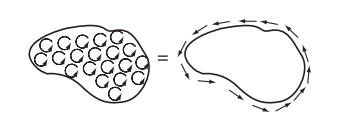
\includegraphics[width=8cm]{Electrodynamics/images/stokes.PNG}
\end{center}

Note that in this theorem, there is ambiguity in picking the direction of $d\vec{a}$ and also the direction to go in the loop integral on the right hand side. However, it suffices to simply be consistent! Use the right hand rule: if your fingers curl around in the direction that $d\vec{\ell}$ travels, your thumb marks the direction of $d\vec{a}$.

Similar to the fundamental theorem for gradients, this gives two important corollaries:

\begin{corollary}
    Surface integrals of curls are independent of the particular surface chosen. In particular
    \[\iint_{\mathcal{S}}(\nabla\times\vec{v})\cdot d\vec{a}\]
    depends only on $\partial\mathcal{S}$.
\end{corollary}

\begin{corollary}
    The integral of curls over a closed surface is equal to zero:
    \[\oiint (\nabla\times\vec{v})\cdot d\vec{a}=0.\]
\end{corollary}

\subsection{Integration by Parts}

Recall that the basic technique of integration by parts utilizes the product rule of derivatives:
\[\frac{d}{dx}(fg)=f\left(\frac{dg}{dx}\right)+g\left(\frac{df}{dx}\right).\]
Integrating both sides from $a$ to $b$ with respect to $dx$ gives
\[\left.fg\right\rvert_{a}^b=\int_a^bf\left(\frac{dg}{dx}\right)dx+\int_a^bg\left(\frac{df}{dx}\right)dx.\]
Rearranging gives
\[\boxed{\int_a^bf\left(\frac{dg}{dx}\right)dx=-\int_a^bg\left(\frac{df}{dx}\right)dx+\left.fg\right\rvert_a^b}.\]
Essentially, if you're integrating the product of one function $f$ and the \textit{derivative} of another function $g$, you can transfer the derivative from $g$ to $f$ at the cost of a boundary term of $fg$ on $\partial([a,b])=\{a,b\}$.

It turns out that you can exploit the product rules of vector calculus in the same way. For example, take the product rule for the divergence of a scalar times a vector:
\[\nabla\cdot(f\vec{v})=f(\nabla\cdot \vec{v})+\vec{v}\cdot(\nabla f).\]
By integrating over a volume, we can abuse Gauss's Law on the left hand side:
\[\iiint_{\mathcal{V}}\nabla\cdot(f\vec{v})d\tau=\iiint_{\mathcal{V}}f(\nabla\cdot \vec{v})d\tau+\iiint_{\mathcal{V}}\vec{v}\cdot(\nabla f)d\tau.\]
The left hand side reduces to
\[\oiint_{\partial\mathcal{V}}f\vec{v}\cdot d\vec{a},\]
so we can write
\[\boxed{\iiint_{\mathcal{V}}f(\nabla\cdot\vec{v})d\tau=-\iiint_{\mathcal{V}}\vec{v}\cdot(\nabla f)d\tau+\oiint_{\partial\mathcal{V}}f\vec{v}\cdot d\vec{a}}.\]
Notice how this has the same form as vanilla integration by parts: we can transfer a derivative (in this case a divergence) from $\vec{v}$ to $f$ (it turns into a gradient) at the cost of a boundary term.

It turns out that integration by parts is actually one of the most powerful tools in vector calculus; there are two other forms presented in the problem below:

\section{Curvilinear Coordinates}

\subsection{Spherical Coordinates}

Recall that instead of Cartesian coordinates, you can also label points in space using \vocab{spherical coordinates} $(r,\theta,\varphi)$. We use physics convention here, where $r=|\vec{r}|$ is the distance to the origin; $\theta$ is the \vocab{polar angle}, the angle between $\vec{r}$ and the $z$-axis; and $\varphi$ is the \vocab{azimuthal angle}, the angle around from the $x$-axis. 

We can easily relate these to Cartesian coordinates:
\[x=r\sin\theta\cos\varphi, \qquad y=r\sin\theta\sin\varphi, \qquad z=r\cos\theta.\]
It turns out that the unit vectors $\hat{r}$, $\hat{\theta}$, and $\hat{\varphi}$ form an orthonormal basis of $\mathbb{R}^3$. Hence you can express any vector $\vec{a}$ as
\[\vec{a}=a_r\hat{r}+a_\theta\hat{\theta}+a_\varphi\hat{\varphi}.\]
It is not too hard to check that
\[
\begin{cases}
\hat{r}=\sin\theta\cos\varphi\cdot \hat{x}+\sin\theta\sin\varphi\cdot\hat{y}+\cos\theta\cdot\hat{z},\\
\hat{\theta}=\cos\theta\cos\varphi\cdot\hat{x}+\cos\theta\sin\varphi\cdot\hat{y}-\sin\theta\cdot\hat{z},\\
\hat{\varphi}=-\sin\varphi\cdot\hat{x}+\cos\varphi\cdot\hat{y}.
\end{cases}
\]

However, there is a very important caveat about this coordinate system! The unit vectors $\hat{r}$, $\hat{\theta}$, and $\hat{\varphi}$ are associated with the \textit{particular point} $P$ that is chosen, and they change direction as $P$ moves around! Therefore, unlike $\hat{x}$, $\hat{y}$, and $\hat{z}$, these basis vectors are not constants. 

For example, do not combine the spherical coordinates of vectors associated with different points (e.g. if $\vec{a}$ and $\vec{b}$) are unit vectors pointing in opposite directions, even though $\vec{a}=\hat{r}$ in its own coordinate system and $\vec{b}=\hat{r}$ in its own coordinate system, we still have that $\vec{a}+\vec{b}=\vec{0}$, not $2\hat{r}$). 

In addition, you need to be careful with differentiating a vector in spherical coordinates, since the unit vectors themselves are functions of position, and need to be differentiated (e.g. $\partial \hat{r}/\partial \theta=\hat{\theta}$).  In addition, you cannot take $\hat{r}$, $\hat{\theta}$, or $\hat{\varphi}$ outside of an integral (e.g. as we did right after Definition \ref{defvolint} in the definition of the volume integral of a vector function).

Due to the setup of spherical coordinates, infinitesimal elements of length are
\[d\vec{\ell}=dr\cdot \hat{r}+rd\theta\cdot \hat{\theta}+r\sin\theta d\varphi\cdot \hat{\varphi}.\]
We call these respective small steps in the $\hat{r}$, $\hat{\theta}$, and $\hat{\varphi}$ directions $d\ell_r=dr$, $d\ell_\theta=rd\theta$, and $d\ell_\varphi=r\sin\theta d\varphi$. 

Similarly, the infinitesimal elements of volume are also different:
\[d\tau=d\ell_r d\ell_\theta d\ell_{\varphi}=r^2\sin\theta drd\theta d\varphi,\]
the product of the scalings $r$ and $r\sin\theta$ that we applied above to the $\hat{\theta}$ and the $\hat{\varphi}$ directions, respectively.

As you can probably imagine, the expression for surface elements is also different, but it's hard to give a general form since it depends on the orientation of the surface. In general, you can always directly analyze the geometry for any given case, but for some examples:
\begin{itemize}
    \item If $r$ is constant (e.g. integrating over a sphere), we have
    \[d\vec{a}=d\ell_\theta d\ell_\varphi\hat{r}=r^2\sin\theta d\theta d\varphi\hat{r}.\]
    \item If the surface lies in the $xy$ plane so that $\theta$ is constant, then
    \[d\vec{a}=d\ell_r d\ell_\varphi\hat{\theta}=rdrd\varphi\hat{\theta}.\]
\end{itemize}
Finally, we note that $r\in [0,\infty)$, $\varphi\in[0,2\pi]$, and $\theta\in[0,\pi]$.

\begin{example}
Find the volume of a sphere of radius $R$.
\end{example}

\begin{proof}[Solution]
Integrate
\begin{align*}
    V&=\iiint_{\mathcal{V}}d\tau=\int_{r=0}^R\int_{\varphi=0}^{2\pi}\int_{\theta=0}^\theta (r^2\sin\theta) d\theta d\varphi dr\\
    &=\left(\int_{0}^R r^2 dr\right)\left(\int_0^{2\pi} d\varphi\right)\left(\int_0^{\pi}\sin\theta d\theta\right)\\
    &=\left(\frac{R^3}{3}\right)(2\pi)(2)=\frac{4}{3}\pi R^3,
\end{align*}
as expected.
\end{proof}

Alright, that finishes a discussion of the \textit{geometry} of spherical coordinates. However, we still need to translate all the vector derivatives we've already discussed. Brute forcing thing would be quite hard, but Appendix describes a much more efficient method, which happens to treat all coordinate systems at once (I haven't taken notes for this, but maybe will in the future).

In any case, let's cut to the chase and just give the formulas:

\begin{proposition}[Vector derivatives in spherical coordinates]
    \begin{itemize}
        \item[]
        \item Gradient:
        \[\nabla T=\frac{\partial T}{\partial r}\hat{r}+\frac{1}{r}\frac{\partial T}{\partial\theta}\hat{\theta}+\frac{1}{r\sin\theta}\frac{\partial T}{\partial\varphi}\hat{\varphi}.\]
        \item Divergence:
        \[\nabla\cdot\vec{v}=\frac{1}{r^2}\frac{\partial}{\partial r}(r^2v_r)+\frac{1}{r\sin\theta}\frac{\partial}{\partial\theta}(\sin\theta v_\theta)+\frac{1}{r\sin\theta}\frac{\partial v_\varphi}{d\varphi}.\]
        \item Curl:
        \begin{align*}
            \nabla\times\vec{v}&=\frac{1}{r\sin\theta}\left[\frac{\partial}{\partial\theta}(\sin\theta v_\varphi)-\frac{\partial v_\theta}{\partial \varphi}\right]\hat{r}+\frac{1}{r}\left[\frac{1}{\sin\theta} \frac{\partial v_r}{\partial \varphi}-\frac{\partial}{\partial r}(rv_\varphi)\right]\hat{\theta}\\
            &+\frac{1}{r}\left[\frac{\partial}{\partial r}(rv_\theta)-\frac{\partial v_r}{\partial \theta}\right]\hat{\varphi}.
        \end{align*}
        \item Laplacian:
        \[\nabla^2 T=\frac{1}{r^2}\frac{\partial}{\partial r}\left(r^2\frac{\partial T}{\partial r}\right)+\frac{1}{r^2\sin\theta}\frac{\partial}{\partial \theta}\left(\sin\theta\frac{\partial T}{\partial \theta}\right)+\frac{1}{r^2\sin^2\theta}\frac{\partial^2T}{\partial \varphi^2}.\]
    \end{itemize}
\end{proposition}

\subsection{Cylindrical Coordinates}

Another method of labeling $\mathbb{R}^3$ is using \vocab{cylindrical coordinates} $(s,\varphi,z)$; where we simply project $P$ down to the $xy$-plane and assign polar coordinates $(s,\varphi)$ to the projection, then let $z$ be the height off the $xy$-plane along the $z$-axis. These relate by
\[x=s\cos\varphi,\qquad y=s\sin\varphi, \qquad z=z.\]
The unit vectors can be written as
\[\begin{cases}
\hat{s}= \cos\varphi\hat{x}+\sin\varphi\hat{y},\\
\hat{\varphi}=-\sin\varphi\hat{x}+\cos\varphi\hat{y},\\
\hat{z}=\hat{z}.
\end{cases}\]
Infinitesimal elements of length are
\[d\vec{\ell}=ds\cdot\hat{s}+sd\varphi\cdot \hat{\varphi}+dz\cdot\hat{z},\]
where the respective small steps in the $\hat{s}$, $\hat{\varphi}$, and $\hat{z}$ directions are $d\ell_s=ds$, $d\ell_\varphi=sd\varphi$, and $d\ell_z=dz$.

Hence, the volume element is
\[d\tau=sdsd\varphi dz.\]
Finally, note that $s\in[0,\infty)$, $\varphi\in[0,2\pi]$, and $z\in(-\infty,\infty)$.

\begin{proposition}[Vector derivatives in cylindrical coordinates]
    \begin{itemize}
        \item[]
        \item Gradient:
        \[\nabla T=\frac{\partial T}{\partial s}\hat{s}+\frac{1}{s}\frac{\partial T}{\partial\varphi}\hat{\varphi}+\frac{\partial T}{\partial z}\hat{z}.\]
        \item Divergence:
        \[\nabla\cdot\vec{v}
        =\frac{1}{s}\frac{\partial}{\partial s}(sv_s)+\frac{1}{s}\frac{\partial v_\varphi}{\partial\varphi}+\frac{\partial v_z}{\partial z}.\]
        \item Curl:
        \[\nabla\times \vec{v}=\left(\frac{1}{s}\frac{\partial v_z}{\partial\varphi}-\frac{\partial v_\varphi}{\partial z}\right)\hat{s}+\left(\frac{\partial v_s}{\partial z}-\frac{\partial v_z}{\partial s}\right)\hat{\varphi}+\frac{1}{s}\left[\frac{\partial}{\partial s}(sv_\varphi)-\frac{\partial v_s}{\partial\varphi}\right]\hat{z}.\]
        \item Laplacian:
        \[\nabla^2 T=\frac{1}{s}\frac{\partial}{\partial s}\left(s\frac{\partial T}{\partial s}\right)+\frac{1}{s^2}\frac{\partial^2T}{\partial\varphi^2}+\frac{\partial^2T}{\partial z^2}.\]
    \end{itemize}
\end{proposition}

\section{The Dirac Delta Function}

\subsection{The Divergence of $\hat{r}/r^2$}

Major apparent paradox: consider 
\[\vec{v}=\frac{1}{r^2}\hat{r}.\]
This function has all arrows pointing outwards; if any vector function would have positive divergence, this is it! Yet, if we calculate the divergence anywhere, we get
\[\nabla\cdot\vec{v}=\frac{1}{r^2}\frac{\partial}{\partial r}\left(r^2\cdot\frac{1}{r^2}\right)=0.\]
What's going on? In fact, it gets even worse if we try applying the divergence theorem. Integrating over a sphere $\mathcal{V}$ of radius $R$ centered at the origin, the surface integral is
\begin{align*}
\oiint_{\partial \mathcal{V}}\vec{v}\cdot d\vec{a}&=\oiint_{\partial\mathcal{V}}\left(\frac{1}{R^2}\hat{r}\right)\cdot (R^2\sin\theta d\varphi d\theta\cdot \hat{r})\\
&=\int_0^\pi \int_0^{2\pi} \sin\theta d\varphi d\theta\\
&=2\pi\cdot\int_0^\pi\sin\theta d\theta=4\pi.
\end{align*}
And yet
\[\iiint_{\mathcal{V}}(\nabla\cdot\vec{v}) d\tau=0,\]
so what's going on? Are we to believe that the divergence theorem is false?

The solution is where $r=0$: the divergence must blow up there. It turns out that $\nabla\cdot \vec{v}$ has the wild property that it vanishes everywhere except one point, yet its integral over any volume including that point is $4\pi$. No ordinary function behaves like this, but it turns out we've stumbled on what is known to physicists as the \vocab{Dirac delta function}.

\subsection{The One-Dimensional Dirac Delta Function}

\begin{definition}
    The \vocab{one-dimensional Dirac delta function}, $\delta(x)$ can be pictured as an infinitely high, infinitesimally narrow ``spike" at the origin, with area 1. Indeed,
    \[\delta(x)=\begin{cases}
    0 & \text{if }x\neq 0\\
    \infty & \text{if }x=0
    \end{cases}\]
    and
    \[\int_{-\infty}^\infty\delta(x)dx=1.\]
    If $x$ has units meters, then $\delta(x)$ has units $(\text{meters})^{-1}$.
\end{definition}

In reality, $\delta(x)$ is not a function since its value at $0$ isn't finite: instead, it's a \vocab{generalized function}, or \vocab{distribution}. It is a \textit{limit} of a \textit{sequence} of functions, say rectangles with height $n$ and width $1/n$, or isosceles triangles of height $n$ and base $2/n$, centered at the origin (as $n\to\infty$).

Note that for an ordinary (continuous) function $f$, we have
\[f(x)\delta(x)=f(0)\delta(x),\]
as their product is 0 whenever $x\neq 0$. Hence
\[\int_{-\infty}^\infty f(x)\delta(x)dx=f(0)\int_{-\infty}^\infty\delta dx=f(0).\]
Under an integral, the delta function ``picks out" the value of $f(x)$ at $x=0$.

We can shift the spike anywhere with $\delta(x-a)$. Then
\[\boxed{\int_{-\infty}^{\infty}f(x)\delta(x-a)dx=f(a)}.\]
This is so important that I've boxed it.

\begin{example}
Evaluate the integral
\[\int_0^3x^3\delta(x-2)dx.\]
What if the upper bound was 1 instead?
\end{example}

\begin{proof}[Solution]
The delta function picks out the value of $x^3$ at $2$, which is $\boxed{8}$. If the upper bound was 1 instead, we wouldn't catch the spike since $2\not\in[0,1]$; hence the integral would be 0.
\end{proof}

So in fact, you should really think of the delta function as something that is \textbf{always intended for use under and integral sign}. In particular, given two expressions $D_1, D_2$ involving delta function, we say that they're considered equal if
\[\int_{-\infty}^\infty f(x)D_1(x)dx=\int_{-\infty}^\infty f(x)D_2(x)dx\]
for \textit{all} functions $f(x)$.

Note that this is because if $D_1$ and $D_2$ were to differ around the neighborhood of some point $x=x'$, then we could just pick $f(x)$ to have a large spike at $x'$, and then the integrals wouldn't be equal anymore.

By $u$-substitution, it can also be shown that
\[\delta(kx)=\frac{1}{|k|}\delta(x).\]
This makes sense, as the factor of $k$ makes it so that you're ``passing through" $\RR$ $k$ times as fast, so you expect to pick up $\frac{1}{|k|}$ as much of it.

\subsection{The Three-Dimensional Delta Function}\label{3ddirac}

If we write $\vec{r}=x\hat{x}+y\hat{y}+z\hat{z}$, then we can generalize:

\begin{definition}
    The \vocab{three-dimensional Dirac delta function} is defined as
    \[\delta^3(\vec{r})=\delta(x)\delta(y)\delta(z).\]
    It is zero everywhere except the origin, where it blows up, and its volume integral is 1:
    \[\iiint_{\mathbb{R}^3}\delta^3(\vec{r})d\tau=\int_{-\infty}^\infty\int_{-\infty}^\infty\int_{-\infty}^\infty\delta(x)\delta(y)\delta(z)=1.\]
\end{definition}

In addition, we have that

\[\boxed{\iiint_{\mathbb{R}^3}f(\vec{r})\delta^3(\vec{r}-\vec{a})d\tau=f(\vec{a})}.\]

To resolve the paradox at the start of this section, we can note that
\[\nabla\cdot\left(\frac{\hat{r}}{r^2}\right)=4\pi\delta^3(\vec{r}).\]
More generally,
\[\boxed{\nabla\cdot\left(\frac{\hat{\scr}}{\scr^2}\right)=4\pi\delta^3(\vec{\scr})},\]
where, recall, $\vec{\scr}=\vec{r}-\vec{r'}$ for some source $\vec{r'}$. Also, since $\nabla\left(\frac{1}{\scr}\right)=-\frac{\vec{\scr}}{\scr^2}$, we have that its Laplacian is
\[\nabla^2\frac{1}{\scr}=-4\pi\delta^3(\vec{\scr}).\]

\begin{example}
Evaluate the integral
\[J=\iiint_{\mathcal{V}}(r^2+2)\nabla\cdot\left(\frac{\hat{r}}{r^2}\right)d\tau,\]
where $\mathcal{V}$ is a ball of radius $R$ centered at the origin.
\end{example}

We present two solutions to this problem: one that demonstrates the Dirac delta function which was just introduced, and another that demonstrates the power of integration by parts.

\begin{proof}[Solution 1]
Rewrite
\[J=\iiint_{\mathcal{V}}(r^2+2)\cdot 4\pi\delta^3(\vec{r})d\tau = 4\pi(0^2+2)=\boxed{8\pi}.\]
\end{proof}

\begin{proof}[Solution 2]
Use integration by parts to transfer the derivative:
\[J=-\iiint_{\mathcal{V}}\nabla(r^2+2)\cdot\frac{\hat{r}}{r^2}d\tau+\oiint_{\partial\mathcal{V}}(r^2+2)\cdot\frac{\hat{r}}{r^2}\cdot d\vec{a}.\]
For the first term, note that the gradient is 
\[\nabla(r^2+2)=\frac{\partial}{\partial r}(r^2+2)\hat{r}=2r\cdot\hat{r},\]
so
\[-\iiint_{\mathcal{V}}\nabla(r^2+2)\cdot\frac{\hat{r}}{r^2}d\tau=-4\pi\int_0^R\frac{2}{r}\cdot r^2dr=-4\pi R^2.\]
Meanwhile, in the surface integral, we have $d\vec{a}=r^2\sin\theta d\varphi d\theta\cdot \hat{r}$ and $r=R$, so it equals
\[\int_{\varphi=0}^{2\pi}\int_{\theta=0}^\pi (R^2+2)d\theta d\varphi=4\pi(R^2+2).\]
Therefore, their sum is
\[J=-4\pi r^2+4\pi(R^2+2)=\boxed{8\pi},\]
which matches.
\end{proof}

\section{The Theory of Vector Fields}

\subsection{The Helmholtz Theorem}

To what extent is a vector function determined by its divergence and curl? If I tell you the divergence of $\vec{F}$ is a certain scalar function $D$,
\[\nabla\cdot\vec{F}=D,\]
and the curl of $\vec{F}$ is a certain vector function $\vec{C}$,
\[\nabla\times\vec{F}=\vec{C},\]
can you determine $\vec{F}$? 

\begin{remark}
Note here that $\vec{C}$ must satisfy $\nabla\cdot\vec{C}=0$, since the divergence of any curl vanishes.
\end{remark}

And the answer is... \textbf{NOPE!} For example, there are many functions with no divergence or curl. To solve such a differential equation (as with any other differential equation), you must be supplied with \textbf{boundary conditions}.  Generally, we simply require that fields go to zero infinitely far away in any direction (from all charges in the problem); with this information, \vocab{Helmholtz theorem} guarantees that the field is uniquely determined by its divergence and curl.

\begin{remark}
In some special cases, charges themselves extend to infinity (e.g. electric field of an infinite plane of a certain charge density). In these cases, the normal boundary conditions no longer apply; instead, one must invoke symmetry arguments to determine the fields uniquely.
\end{remark}

\subsection{Potentials}

Recall that the curl of any gradient is equal to zero. Well, it turns out that it works the other away around too.

\begin{definition}
If a vector field $\vec{F}$ has a curl that vanishes everywhere, then it can be written as the gradient of a scalar function $V$ that we call its \vocab{scalar potential}:
\[\nabla\times \vec{F}=\vec{0}\quad\Longleftrightarrow\quad \vec{F}=-\nabla V.\]
\end{definition}

\begin{remark}
The negative sign is purely for convention, so that forces push you to places of \textit{lower} potential (energy).
\end{remark}

This definition works because of the following theorem:

\begin{theorem}[Irrotational fields]\label{irrotfields}
    The following are equivalent:
    \begin{enumerate}[(1)]
        \item $\nabla\times\vec{F}=\vec{0}$ everywhere.
        \item $\int_{\vec{a}}^{\vec{b}}\vec{F}\cdot d\vec{\ell}$ is independent of path, for any given endpoints.
        \item $\oint \vec{F}\cdot d\vec{\ell}=0$ for any closed loop.
        \item $\vec{F}$ is the gradient of some scalar function: $\vec{F}=-\nabla V$.
    \end{enumerate}
\end{theorem}

The scalar potential is not unique: you can add any constant to $V$ and the gradient will be unaffected.

\begin{definition}
If a vector field $\vec{F}$ has divergence that vanishes everywhere, then it can be written as the curl of a vector function $\vec{A}$ that we call its \vocab{vector potential}:
\[\nabla\cdot\vec{F}=0\quad\Longleftrightarrow\quad \vec{F}=\nabla\times\vec{A}.\]
\end{definition}

This definition also works because of the following (similar) theorem:
\begin{theorem}[Solenoidal (incompressible) fields]
    The following are equivalent:
    \begin{enumerate}[(1)]
        \item $\nabla\cdot\vec{F}=0$ everywhere.
        \item $\iint \vec{F}\cdot d\vec{a}$ is independent of surface, for any given boundary line.
        \item $\oiint \vec{F}\cdot d\vec{a}=0$ for any closed surface.
        \item $\vec{F}$ is the curl of some vector function: $\vec{F}=\nabla\times\vec{A}$.
    \end{enumerate}
\end{theorem}

This vector potential is also not unique: the gradient of any scalar function can be added to $\vec{A}$ without affecting the curl.

It turns out that in all cases, a vector field $\vec{F}$ can be written as the gradient of a scalar plus the curl of a vector:
\begin{moral}
We can always write
\[\vec{F}=-\nabla V+\nabla\times\vec{A}.\]
\end{moral}


\chapter{Electrostatics}

\section{The Electric Field}

\subsection{Introduction}

The fundamental problem in electrodynamics is how \vocab{source charges} $q_1,q_2,\dots$ (whose positions are \textit{given} as functions of time) affect a \vocab{test charge} $Q$ (whose trajectory is to be \textit{calculated}).

The \vocab{law of superposition} helps: the net force $\vec{F}$ on $Q$ is just the vector sum of the forces $\vec{F}_i$ from $q_i$ on $Q$:
\[\vec{F}=\sum_i \vec{F}_i.\]

Sadly, each individual force $\vec{F}_i$ is not easy to calculate, either. Indeed, it depends not only on the separation distance $\scr$, but also \textit{both} their velocities and on the \textit{acceleration} of $q$. Further, electromagnetic ``news" only propagates at the speed of light, so we need to consider \textit{not} what each $q_i$ is doing now, but what it was doing at some slightly earlier time.

So we need to simplify the problem. In \vocab{electrostatics}---as the name suggests---we take all the source charges $q_i$ to be static, or stationary (the test charge $Q$ can still move).

\subsection{Coulomb's Law}

Recall:

\begin{theorem}[Coulomb's Law]
The force of a stationary charge $q$ on a test charge $Q$ that is $\scr$ away is given by
\[\vec{F}=\frac{1}{4\pi\varepsilon_0}\frac{qQ}{\scr^2}{\hat{\scr}}.\]
This is confirmed by experiments. 
\end{theorem}

\begin{definition}
The constant here is
\[\varepsilon_0=8.85\times 10^{-12}\frac{\text{C}^2}{\text{N}\cdot\text{m}^2},\]
called the \vocab{permittivity of free space}.
\end{definition}

Notice that the force $\vec{F}$ is repulsive if $q$ and $Q$ have the same sign, and attractive if they have different signs. Indeed, $\vec{\scr}$ points from $q$ to $Q$.

\subsection{The Electric Field}

Now suppose we have $n$ source charges $q_1,q_2,\dots,q_n$, with respective vectors $\vec{\scr_1},\vec{\scr_2},\dots,\vec{\scr_n}$ to a test charge $Q$. Then, by the superposition principle, we have that
\[\vec{F}=\sum_{i=1}^n\vec{F}_i=\frac{Q}{4\pi\varepsilon_0}\sum_{i=1}^n\frac{q}{\scr_i^2}\hat{\scr_i}.\]
Notice how this quantity is proportional to $Q$, so we can define another vector field that depends \textit{only} on the source charges:
\begin{definition}
We define the \vocab{electric field} generated by source charges $q_1,\dots,q_n$ at a point $\vec{r}$ as
\[\vec{E}(\vec{r}):=\frac{1}{4\pi\varepsilon_0}\sum_{i=1}^n\frac{q_i}{\scr_i^2}\hat{\scr_i}.\]
\end{definition}
Then, the force of a test charge $Q$ placed at $\vec{r}$ is $\vec{F}=Q\vec{E}$, by the definition of $\vec{E}$. Further, since $\vec{E}$ is independent of any test charges $Q$, we can imagine it as an actual ``real" physical field that permeates space, and when test charges $Q$ are placed in the field they get pushed along (or against) the electric field.

\subsection{Continuous Charge Distribution}\label{contchardist}

We have only covered the case where the source is a collection of discrete point charges: to cover the continuous case, we need to turn our sum into an integral:
\[\vec{E}(\vec{r})=\frac{1}{4\pi\varepsilon_0}\int \frac{dq}{\scr^2}\hat{\scr}.\]
\begin{itemize}
    \item If the charge is spread over a line, with linear charge density $\lambda$, then $dq=\lambda d\ell'$, so
    \[\vec{E}(\vec{r})=\frac{1}{4\pi\varepsilon_0}
    \int\frac{\lambda(\vec{r'})}{\scr^2}\hat{\scr}d\ell'.\]
    \item If the charge is spread over a plane, with surface charge density $\sigma$, then $dq=\sigma da'$, so
    \[\vec{E}(\vec{r})=\frac{1}{4\pi\varepsilon_0}\int\frac{\sigma(\vec{r'})}{\scr^2}\hat{\scr}da'.\]
    \item If the charge is spread over a volume, with volume charge density $\rho$, then $dq=\rho d\tau'$, so
    \[\boxed{\vec{E}(\vec{r})=\frac{1}{4\pi\varepsilon_0}\int\frac{\rho(\vec{r'})}{\scr^2}\hat{\scr}d\tau'}.\]
\end{itemize}

Often, the final boxed equation is referred to as ``Coulomb's Law": it is not far from our original formulation, and volume charge distributions are common.

\section{Divergence and Curl of Electrostatic Fields}

\subsection{Field Lines, Flux, and Gauss' Law}

In principle, we are done with electrostatics: just compute the boxed integral above to find the electric field generated by the source charges; we know that a test charge $Q$ will simply receive a force $\vec{F}=Q\vec{E}$ at a point with electric field $\vec{E}$.

However, that integral is often intractable, so much of electrostatics is actually concerned with \textbf{assembling a bag of tools and tricks} to avoid them.

One tool to get a feel for electric fields is through \vocab{field lines}. We consider the case of a single point charge $q$ at the origin; shown below are (a) some vectors in the electric field and (b) electric field lines.

\begin{center}
    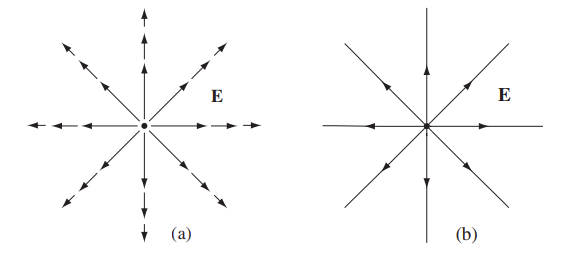
\includegraphics[width=12cm]{Electrodynamics/images/fig2.12.PNG}
\end{center}

It may seem like we lost some information: the strength of the field. However, we actually haven't! It turns out the magnitude of the field is indicated by the \textbf{density} of the field lines. However, the picture is actually a bit deceptive when drawn in two dimensions: it seems like the field drops with $1/r$; however, in three dimensions, we do get the correct $1/r^2$.

Note that charges must have a number of field lines emanating/terminating at it proportional to the magnitude of the charge. Further, electric field lines cannot terminate at any points other than charges (else $\nabla\cdot\vec{E}=0$, something we'll prove later, would be violated): they must start/end at charges or at infinity. Further, field lines cannot cross (otherwise the electric field at that point would have two directions!). Depicted below are the field lines for an electric dipole.

\begin{center}
    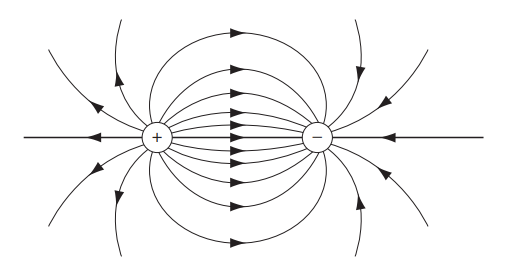
\includegraphics[width=10cm]{Electrodynamics/images/fig2.13.PNG}
\end{center}

Further, using this model, there's a simple interpretation for the \textit{flux} of $\vec{E}$ through a surface $\mathcal{S}$:
\[\Phi_E=\iint_{\mathcal{S}}\vec{E}\cdot d\vec{a}\]
is simply the (signed) number of electric field lines passing through $\mathcal{S}$.

This suggests that the flux through a \textit{closed} surface should measure the total charge inside the surface; in particular, charges outside should have no affect on the flux since any field lines that enter simply exit again.

This is the essence of \vocab{Gauss's law}.

\begin{theorem}[Gauss's Law]
    For any closed surface $\mathcal{S}$, we have
    \[\oiint_{\mathcal{S}}\vec{E}\cdot d\vec{a}=\frac{Q_{\text{enc}}}{\varepsilon_0},\]
    where $Q_{\text{enc}}$ is the total charge enclosed within $\mathcal{S}$.
\end{theorem}

Note that since Newton's law of gravitation also obeys $1/r^2$ fall-off, it will also obey an analogous Gauss's law.

To turn this into differential form, we can rewrite the left hand side using the divergence theorem:
\[\oiint_{\mathcal{S}}\vec{E}\cdot d\vec{a}=\iiint_{\mathcal{V}}(\nabla\cdot \vec{E})d\tau\]
where $\partial\mathcal{V}=\mathcal{S}$; i.e. $\mathcal{V}$ is the interior of $\mathcal{S}$. In addition, we can write
\[\frac{Q_{\text{enc}}}{\varepsilon_0}=\iiint_{\mathcal{V}}\rho d\tau.\]
Hence.
\[\iiint_{\mathcal{V}}(\nabla\cdot\vec{E})d\tau=\iiint_{\mathcal{V}}\left(\frac{\rho}{\varepsilon_0}\right)d\tau.\]
However, since this holds true for \textit{any} volume of choice $\mathcal{V}$, the integrands must also be equal.

\begin{theorem}[Gauss's Law in Differential Form]
    We have that
    \[\nabla\cdot\vec{E}=\frac{\rho}{\varepsilon_0}.\]
\end{theorem}

\subsection{The Divergence of $\vec{E}$}

Let's calculate the divergence of $\vec{E}$ directly from the boxed equation in Section \ref{contchardist}:
\[\vec{E}(\vec{r})=\frac{1}{4\pi\varepsilon_0}\iiint_{\mathbb{R}^3}\frac{\hat{\scr}}{\scr^2}\rho(\vec{r'})d\tau'.\]
Since the only dependence on $\vec{r}$ is in $\vec{\scr}=\vec{r}-\vec{r'}$, and the divergence is linear, we can write
\[\nabla\cdot\vec{E}=\frac{1}{4\pi\varepsilon_0}\iiint_{\mathbb{R}^3}\nabla\cdot\left(\frac{\hat{\scr}}{\scr^2}\right)\rho(\vec{r'})d\tau'.\]
Recall that in Section \ref{3ddirac} we showed that $\nabla\cdot\left(\frac{\hat{\scr}}{\scr^2}\right)=4\pi\delta^3(\vec{\scr})$,
so
\[\nabla\cdot\vec{E}=\frac{1}{4\pi\varepsilon_0}\iiint_{\mathbb{R}^3}4\pi\delta^3(\vec{r}-\vec{r'})\rho(\vec{r'})d\tau'=\frac{\rho(\vec{r})}{\varepsilon_0},\]
as desired.

We can recover the original form of Gauss's law by simply integrating over a volume $\mathcal{V}$.

\subsection{Applications of Gauss's Law}

Gauss's law is \textbf{extraordinarily powerful}, especially when symmetry permits. 

\begin{definition}
When we apply Gauss's law over a closed surface $\mathcal{S}$ that the boundary of some volume, we generally refer to that surface as a \vocab{Gaussian surface}.
\end{definition}

\begin{example}[Electric Field of Ball]
Find the field outside a uniformly charged solid ball of radius $R$ and total charge $q$.
\end{example}

\begin{proof}
Suppose we wish to find the field $r$ away from the center: then, draw our Gaussian surface $\mathcal{S}$ as a sphere of radius $r$ that is concentric with our solid charged ball.

Gauss's law tells us that 
\[\oiint_{\mathcal{S}}\vec{E}\cdot d\vec{a}=\frac{Q_{enc}}{\varepsilon_0}=\frac{q}{\varepsilon_0}.\]
Now, by spherical symmetry, the electric fields $\vec{E}$ along $\mathcal{S}$ must all point directly outward (parallel to $d\vec{a}$), and have equal magnitude; hence,
\[E\cdot 4\pi r^2=\frac{q}{\varepsilon_0}\implies \vec{E}=\boxed{\frac{1}{4\pi \varepsilon_0}\frac{q}{r^2}\hat{r}}.\]
\end{proof}

This is actually the exact same as the electric field generated by a point charge $q$ placed at the center of the sphere, which is true by the shell theorem. 

In general, there are two types of symmetry: spherical symmetry and cylindrical symmetry. In the first case, make your Gaussian surface a concentric sphere; in the second, make your Gaussian surface a coaxial cylinder.

\begin{exercise}
A long cylinder carries a charge density that is proportional to the distance from the axis: $\rho=ks$, for some constant $k$. Find the electric field inside this cylinder.
\end{exercise}

\begin{exercise}[Electric Field of Plane]
An infinite plane carries a uniform surface charge $\sigma$. Find its electric field.
\end{exercise}

\begin{exercise}[Parallel Plate Capacitor]
Two infinite parallel planes carry equal but opposite uniform charge densities $\pm \sigma$. Find the field in each of the three regions: (i) to the left of both, (ii) between them, (iii) to the right of both.
\end{exercise}

\subsection{The Curl of $\vec{E}$}

We can calculate the curl of $\vec{E}$ in the simple case of a point charge at the origin:
\[\vec{E}=\frac{1}{4\pi\varepsilon_0}\frac{q}{r^2}\hat{r}.\]
If we calculate the line integral 
\[\int_{\vec{a}}^{\vec{b}}\vec{E}\cdot d\vec{\ell}\]
of this field from point $\vec{a}$ to point $\vec{b}$, remember that we can write
\[d\vec{\ell}=dr\hat{r}+rd\theta\hat{\theta}+r\sin\theta d\varphi \hat{\varphi}.\]
Hence,
\[\vec{E}\cdot d\vec{\ell}=\frac{1}{4\pi\varepsilon_0}\frac{q}{r^2}dr.\]
Hence
\[\int_{\vec{a}}^{\vec{b}}\vec{E}\cdot d\vec{\ell}=\frac{1}{4\pi\varepsilon_0}\int_{\vec{a}}^{\vec{b}}\frac{q}{r^2}dr=\frac{1}{4\pi\varepsilon_0}\left(\frac{q}{r_a}-\frac{q}{r_b}\right),\]
where $r_a,r_b$ are the distances of $\vec{a},\vec{b}$ from the origin, respectively.

Therefore, the line integral between two points $\vec{a}$ and $\vec{b}$ doesn't depend on the particular path chosen; so the loop integral of $\vec{E}$ is also equal to zero:
\[\oint \vec{E}\cdot d\vec{\ell}=0\]
for any closed loop. Therefore, by Stokes' Theorem, we have that $\nabla\times\vec{E}=\vec{0}$.

Since $\nabla$ is linear, this also applies for any set of discrete point charges by the superposition principle.

\section{Electric Potential}

\subsection{Introduction to Potential}

Electric fields aren't just any old vector fields. They are in a very special class of vector functions: ones that have no curl anywhere, i.e. $\nabla\times\vec{E}=\vec{0}$. However, becuase of this, we can use Theorem \ref{irrotfields} to reduce the \textit{vector} problem of finding $\vec{E}$ to the \textit{scalar} problem.

\begin{definition}
Since $\nabla\times\vec{E}=\vec{0}$, there exists some scalar field $V$ such that $\vec{E}=-\nabla V$. We call $V$ the \vocab{electric potential}. 
\end{definition}

If we agree on some standard reference point $\mathcal{O}$ in the plane, then it turns out the function
\[V(\vec{r}):=-\int_{\mathcal{O}}^{\vec{r}} \vec{E}(\vec{r'})\cdot d\vec{\ell'}.\]
Since $\vec{E}$ is path-independent, this integral depends only on $\vec{r}$. In particular, the potential \textit{difference} between any two points $\vec{a}$ and $\vec{b}$ is simply
\[V(\vec{b})-V(\vec{a})=-\int_{\vec{a}}^{\vec{b}}\vec{E}\cdot d\vec{\ell}.\]
This is equivalent to $\vec{E}=-\nabla V$ by the fundamental theorem of gradients:
\[V(\vec{b})-V(\vec{a})=\int_{\vec{a}}^{\vec{b}}(\nabla V)\cdot d\vec{\ell}.\]

\subsection{Comments on Potential}

\paragraph{The name.} The name ``potential" invariably reminds you of ``potential energy." There is a connection, but they are completely different terms that should have different names. A surface over which the potential is constant is called an \vocab{equipotential}.

\paragraph{Advantage of the potential formulation.} If you know $V$, you can easily get $\vec{E}$ just by taking the gradient:
\[\vec{E}=-\nabla V.\]
Yet $\vec{E}$ is a \textit{vector} quantity while $V$ is a \textit{scalar} quantity. How can \textit{one} function $V$ contain all the information for the \textit{three} components of $\vec{E}$.

The reason, as it turns out, is that $\vec{E}$ is a very special type of function, being irrotational. Indeed, the condition $\nabla\times \vec{E}$, in components, translates to
\[\frac{\partial E_x}{\partial y}=\frac{\partial E_y}{\partial x}, \qquad \frac{\partial E_z}{\partial y}=\frac{\partial E_y}{\partial z}, \qquad \frac{\partial E_x}{\partial z}=\frac{\partial E_z}{\partial x}.\]

\paragraph{The reference point.} There is an ambiguity in defining $V$, based on the choice of reference point $\mathcal{O}$. However, altering the reference point amounts to just shifting by a constant. 

In this sense, potential is a lot like altitude: if I asked you the height of something, you'd probably give it to me in terms of its height above sea level, but it would be just as valid to measure with respect to New York, or Greenwich, or wherever. Shifting by a constant doesn't matter; rather, the only quantity that actually matters is the \textit{difference} in altitude between any two points.

Nonetheless, there is a natural spot for $\mathcal{O}$ in electrostatics: and that is a point infinitely far from any charge. So, we set the zero of potential at infinity. Once again, this convention fails if the charge itself extends to infinity; in these cases, the potential often blows up. The remedy is to pick some other point in space as the reference point. Also note that in real life, we never have to deal with this issue.

\paragraph{Potential obeys the superposition principle.} Since the electric field obeys this principle and $\nabla$ is linear, so should the potential. However, it's even better now since it's an \textit{ordinary} sum of scalars, not vectors.

\paragraph{Units of potential.} As electric fields are newtons per coulomb, potential is newton-meters per coulomb, or joules per coulomb. We call this unit a \vocab{volt}.

\begin{example}
Find the potential inside and outside a spherical shell of radius $R$ that carries a uniform surface charge, and total charge $q$.
\end{example}

\begin{proof}[Solution]
    Recall that the electric field generated by the sphere is
    \[\vec{E}(\vec{r})=\begin{cases}
        \frac{1}{4\pi \varepsilon_0}\frac{q}{r^2}\hat{r} & \text{if }r>R,\\
        0 & \text{otherwise}.
    \end{cases}\]
    For points outside of the sphere we integrate
    \[V(r)=-\int_\infty^{\vec{r}}\vec{E}\cdot d\vec{\ell}=-\frac{1}{4\pi \varepsilon_0}\int_\infty^r \frac{q}{r'^2}dr'=\frac{1}{4\pi\varepsilon_0}\frac{q}{r} \qquad (r>R).\]
    For points inside the sphere, note that $\nabla V=\vec{0}$ inside, so we simply have 
    \[V(r)=\frac{1}{4\pi\varepsilon_0}\frac{q}{R}\qquad (r<R).\]
\end{proof}

\subsection{Poisson's Equation and Laplace's Equation}

Recall that we can write $\vec{E}=-\nabla V$. However, also recall that we've determined that
\[\nabla\cdot \vec{E}=\frac{\rho}{\varepsilon_0}\qquad \text{and}\qquad\nabla\times\vec{E}=\vec{0}.\]
Substituting in $V$ gives
\[\nabla\cdot (\nabla V)=-\frac{\rho}{\varepsilon_0}.\]
Recall that the divergence of the gradient is the \textit{Laplacian}. This gives \vocab{Poisson's Equation}.

\begin{theorem}[Poisson's Equation]
We have
\[\nabla^2 V=-\frac{\rho}{\varepsilon_0}.\]
\end{theorem}

In regions with no charge, this reduces to \vocab{Laplace's Equation},
\[\nabla^2 V=0.\]

What about the fact that $\vec{E}$ is irrotational? Sadly, it doesn't give anything, since the curl of a gradient (of $V$) should always equal $\vec{0}$ anyway.

\subsection{The Potential of a Localized Charge Distribution}

Usually, we want to find $\vec{E}$ from $V$, and $V$ from the charge distribution $\rho$. Sadly, Poisson's Equation is the wrong way around: we can take the Laplacian of $V$ to get $\rho$. Is there some way we can ``invert" Poisson's equation?

Recall that a point charge $q$ at the origin generates a potential
\[V(r)=\frac{1}{4\pi\varepsilon_0}\frac{q}{r}.\]
It turns out that we can generalize this to arbitrary charge distributions:
\[V(\vec{r})=\frac{1}{4\pi\varepsilon_0}\int\frac{1}{\scr}dq.\]
For volume charge distributions, $dq=\rho\cdot d\tau'$, so
\[\boxed{V(\vec{r})=\frac{1}{4\pi\varepsilon_0}\iiint\frac{\rho(\vec{r'})}{\scr}d\tau'}.\]
This is a solution to Poisson's equation for a localized charge distribution. Similarly, for surface and line charge distributions we get potentials
\[V=\frac{1}{4\pi\varepsilon_0}\int\frac{\lambda(\vec{r'})}{\scr}d\ell'\qquad\text{and}\qquad V=\frac{1}{4\pi\varepsilon_0}\iint\frac{\sigma(\vec{r'})}{\scr}da'.\]
Recall once again that this section depends on the fact that the reference point is at infinity.

\subsection{Boundary Conditions}

We have covered the three fundamental quantities in electrostatics: $\rho$, $\vec{E}$, and $V$. We have also derived all six formulas interrelating them, summarized below. All six of these formulas followed from two experimental observations: (1) the principle of superposition and (2) Coulomb's law.

\begin{center}
    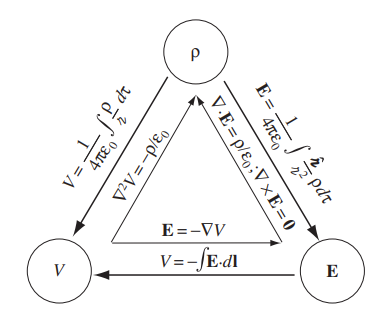
\includegraphics[width=10cm]{Electrodynamics/images/fig2.35.PNG}
\end{center}

Now onto the point of this section: what happens to $\vec{E}$ and $V$ when you cross a \textit{boundary}, i.e. a surface with charge density $\sigma$. 

It is simple to determine this for $\vec{E}$ using Gauss's law: simply draw a really thin wafer of area $A$ and thickness $\epsilon$ containing the surface; then
\[\oiint_{\mathcal{S}}\vec{E}\cdot d\vec{a}=\frac{Q_{\text{enc}}}{\varepsilon_0}=\frac{\sigma A}{\varepsilon_0}.\]
Even if there are other electric charges in the area, the flux through the sides of the pillbox is 0 as we take $\epsilon\to 0$. Hence, the difference in the normal component of the electric field below and the \textit{normal} component (obtained after dotting with $d\vec{a}$) of the electric field above is $\frac{\sigma}{\varepsilon_0}$. Note that this is true for a single infinitely flat plane with surface charge density $\sigma$ as well: the electric fields are both of magnitude $\frac{\sigma}{2\varepsilon_0}$, but pointing in opposite directions.

However, the \textit{tangential} component of $\vec{E}$ is \textit{always} continuous. After all, the loop integral of $\vec{E}$ is always $0$, so if we considered a small loop that is the along the side of the pillbox (so length $\ell$ parallel to the surface and length $\epsilon$ through the surface), then we see that the tangential components must be equal (since their difference is 0).

Hence, we can summarize:
\[\vec{E}_{\text{above}}-\vec{E}_{\text{below}}=\frac{\sigma}{\varepsilon_0}\hat{n},\]
where $\hat{n}$ is a unit vector pointing from below to above.

On the other hand, the potential is continuous across \textit{any} boundary, since the difference in $V$ is given by the path integral of $\vec{E}$, but since the path length shrinks to zero, so too does the integral:
\[V_{\text{above}}-V_{\text{below}}=-\int_{\text{below}}^{\text{above}}\vec{E}\cdot d\vec{\ell}=0.\]

The \textit{gradient} of $V$ keeps the discontinuity though, so
\[\nabla V_{\text{above}}-\nabla V_{\text{below}}=-\frac{\sigma}{\varepsilon_0}\hat{n}.\]
More conveniently, we can consider the $\hat{n}$ component of both sides by taking the dot product with $\hat{n}$, recalling that the dot product of the gradient of $V$ with a unit vector gives the rate of change of $V$ along the direction of that unit vector:
\[\frac{\partial V}{\partial n}=(\nabla V)\cdot\hat{n};\]
in this case, we call it the \vocab{normal derivative} of $V$, i.e. the rate of change of $V$ in the direction perpendicular (normal) to the surface. Hence, we can write
\[\frac{\partial V_{\text{above}}}{\partial n}-\frac{\partial V_{\text{below}}}{\partial n}=-\frac{\sigma}{\varepsilon_0}.\]

\section{Work and Energy in Electrostatics}

\subsection{The Work It Takes to Move a Charge}

Suppose we have a \textit{stationary} configuration of source charges, and want to move a test charge $Q$ from $\vec{a}$ to $\vec{b}$. How much work will we have to do?

Well, the force at any point is given by $\vec{F}=Q\vec{E}$; so you need to exert $-Q\vec{E}$. Hence the needed work is
\[W=\int_{\vec{a}}^{\vec{b}}\vec{F}\cdot d\vec{\ell}=-Q\int_{\vec{a}}^{\vec{b}}\vec{E}\cdot d\vec{\ell}=Q[V(\vec{b})-V(\vec{a})].\]
As $\nabla\times \vec{E}=\vec{0}$, this answer is independent of the path from $\vec{a}$ to $\vec{b}$: therefore, we call the electrostatic force \textit{conservative}.

Hence,
\[V(\vec{b})-V(\vec{a})=\frac{W}{Q}.\]
This gives us another view of potential:
\begin{moral}
The potential difference between points $\vec{a}$ and $\vec{b}$ is equal to the work per unit charge required to carry a particle from $\vec{a}$ to $\vec{b}$.
\end{moral}
In particular, if you want to bring $Q$ in from far away at stick it at $\vec{r}$, you must do work $W=Q\cdot V(\vec{r})$ (as we set our reference point at infinity). In this sense, potential is \textit{potential energy per unit charge} of a single particle moving within a field generated by stationary source charges.

\subsection{The Energy of a Point Charge Distribution}

But what we want to assemble an entire \textit{collection} of point charges? How much work would we need?

The first charge $q_1$ takes zero work: there's nothing to help or fight against. Bringing in $q_2$ will cost $q_2V_1(\vec{r_2})$, where $V_1$ is the potential due to $q_1$, which is then evaluated at $\vec{r_2}$:
\[W_2=\frac{1}{4\pi \varepsilon_0}\frac{q_1q_2}{\scr_{12}},\]
where $\scr_{12}$ is the distance from $\vec{r_1}$ to $\vec{r_2}$. Moving in $q_3$ then takes
\[W_3=\frac{1}{4\pi\varepsilon_0}\frac{q_1q_3}{\scr_{13}}+\frac{1}{4\pi\varepsilon_0}\frac{q_2q_3}{\scr_{23}},\]
and so on. Continuing this pattern, the total work necessary is
\[W=\frac{1}{4\pi \varepsilon_0}\sum_{i=1}^n\sum_{j=i+1}^n\frac{q_iq_j}{\scr_{ij}}=\frac{1}{8\pi\varepsilon_0}\sum_{i=1}^n\sum_{j\neq i}^n\frac{q_iq_j}{\scr_{ij}}.\]
This is equal to
\begin{equation}\label{pointchargeenergy}
\frac{1}{2}\sum_{i=1}^nq_i\left(\sum_{j\neq i}^n\frac{1}{4\pi\varepsilon_0}\frac{q_i}{\scr_{ij}}\right)=\frac{1}{2}\sum_{i=1}^nq_iV(\vec{r_i}).
\end{equation}
This is exactly half of what you'd expect if you just added the work of placing any point charge into the configuration (holding everything else and their generated potential fixed).

This value represents the energy stored in the system of charges (avoiding the annoying term \textit{``potential" energy}).

\subsection{The Energy of a Continuous Charge Distribution}

For a volume charge density $\rho$, this becomes
\[W=\frac{1}{2}\iiint_{\mathbb{R}^3}\rho Vd\tau.\]
There is actually a wonderful way to rewrite this equation to get rid of $\rho$ and $V$ in place of $\vec{E}$. First, use Gauss's law to convert $\rho$ to $\vec{E}$:
\[\rho=\varepsilon_0
\nabla\cdot \vec{E}\implies W=\frac{\varepsilon_0}{2}\iiint_{\mathbb{R}^3}(\nabla\cdot \vec{E})Vd\tau.\]
Now, use integration by parts to transfer the derivative from $\vec{E}$ to $V$:
\[W=\frac{\varepsilon_0}{2}\left[-\iiint_{\mathbb{R}^3}E\cdot(\nabla V)d\tau+\oiint_{\partial \mathbb{R}^3}V\vec{E}\cdot d\vec{a}\right].\]
Wait a second... what's $\partial \RR^3$? Well... if we expand the volume containing charge over and over then the surface integral will drop to $0$ since area grows with $r^2$ but $V$ falls off with $1/r$ and $\vec{E}$ falls off with $1/r^2$.

Now we can use $\nabla V=-\vec{E}$ to get
\begin{equation}\label{energyelectric}
W=\frac{\varepsilon_0}{2}\iiint_{\RR^3}E^2d\tau.
\end{equation}
The energy stored in an electric field per unit volume, then, is $\frac{\varepsilon_0E^2}{2}$.

\subsection{Comments on Electrostatic Energy}

\paragraph{A perplexing ``inconsistency".} The equation 
\[W=\iiint\frac{\varepsilon_0 E^2}{2}d\tau\]
seems to imply that the energy of a stationary charge distribution is \textit{always positive}. Yet the energy of two equal but opposite charges a distance $\scr$ apart is apparently negative quantity $-(1/4\pi\varepsilon_0)(q^2/\scr)$, according to Equation \ref{pointchargeenergy}.

What's going on? Well, \textit{both are correct}. The problem here is that the energy in $-(1/4\pi\varepsilon_0)(q^2/\scr)$ \textbf{doesn't take into account the energy necessary to \textit{create} the point charges} (it supposes the point charges are already given, we're just assembling them), while Equation \ref{energyelectric} does. 

This is good, in fact, as the energy of a point charge is actually \textit{infinite}. By Equation \ref{energyelectric},
\begin{align*}
W&=\frac{\varepsilon_0}{2}\iiint_{\mathbb{R}^3}\frac{1}{(4\pi\varepsilon_0)^2}\cdot \frac{q^2}{r^4}d\tau\\
&=\frac{q^2}{32\pi^2\varepsilon_0}\int_{\varphi=0}^{2\pi}\int_{\theta=0}^\pi\int_{r=0}^\infty \frac{1}{r^4}\cdot r^2\sin\theta drd\theta d\varphi.\\
&=\frac{q^2}{8\pi\varepsilon_0}\int_0^\infty \frac{1}{r^2}dr=\infty.
\end{align*}

So Equation \ref{energyelectric} is more \textit{complete} in giving the total energy stored in the charge configuration. Yet for point charges, as we've seen, we definitely shouldn't include this, so Equation \ref{pointchargeenergy} assumes the point charges are already made (e.g. electrons), and cannot be taken apart. So the energy inside them doesn't matter.

\paragraph{Where is the energy stored?} Is the energy stored in the charge, or in the field? Presently, this is an unanswerable question: we can compute \textit{what} the total energy is, and several ways to compute it, but worrying \textit{where} it is is irrelevant. In radiation theory and general relativity, it is useful to regard the energy as stored in the field with energy density $\frac{\varepsilon E^2}{2}$ per unit volume.

However, in electrostatics, we can just as well say that the energy is stored in the charge, with density $\frac{1}{2}\rho V$.

\paragraph{The superposition principle.} Because electrostatic energy is \textit{quadratic} in the fields, it does \textit{not} obey a superposition principle. The energy of a compound system is \textit{not} the sum of the energies of its parts considered equally, as there are cross terms:
\[W_{\text{tot}}=\frac{\varepsilon_0}2\iiint (\vec{E_1}+\vec{E_2})^2d\tau=W_1+W_2+\varepsilon_0\iiint \vec{E_1}\cdot\vec{E_2}d\tau.\]
For example, if you double the charge everywhere, you quadruple the total energy.



\chapter{Potentials}\label{potentials}

\section{Laplace's Equation}

\subsection{Introduction}

We are interested in the differential form of Poisson's equation,
\[\nabla^2V=-\frac{\rho}{\varepsilon_0},\]
which is equivalent to the integral form
\[V(\vec{r})=\frac{1}{4\pi\varepsilon_0}\iiint\frac{\rho(\vec{r'})}{\scr}d\tau'\]
if we're given boundary conditions.

More often, we're interested in finding the potential in regions where $\rho=0$. Here, Poisson's equation reduces to Laplace's equation
\[\nabla^2V=0,\qquad\text{or}\qquad \frac{\partial^2V}{\partial x^2}+\frac{\partial^2V}{\partial y^2}+\frac{\partial^2V}{\partial z^2}=0.\]
This is so fundamental the subject that one might say electrostatics \textit{is} the study of Laplace's equation. This equation plays a role in many branches of physics and mathematics.

\begin{definition}
A solution to Laplace's equation is called a \vocab{harmonic function}.
\end{definition}

To get a feel for these harmonic functions, we will begin in lower dimensions.

\subsection{Laplace's Equation in One Dimension}

In one dimension, Laplace's equation is
\[\frac{d^2V}{dx^2}=0.\]
This means the derivative $\frac{dV}{dx}$ is constant over $x$; hence, the general solution is a straight line
\[V(x)=mx+b.\]
Since it contains two free variables, this solution is appropriate for a second-order differential equation (as we need to specify some pair of either $V$ or $V'$ as initial conditions).

There are two important features of this result that generalize nontrivially in higher dimensions:
\begin{enumerate}
    \item $V(x)$ is the \textit{average} of $V(x+a)$ and $V(x-a)$, for \textit{any} $a$:
    \[V(x)=\frac{1}{2}[V(x+a)+V(x-a)].\]
    Hence, Laplace's equation tells you to average values; if you're given some endpoints as boundary conditions, harmonic functions are, in this sense, as \textit{boring as they possibly could be} yet still fit the endpoints.
    \item Laplace's equation allows \textit{no local maxima or minima}; the only extreme values of $V$ can occur at the endpoints. This is a consequence of the above property: if there were a local maxima then it wouldn't be an average of its neighbors.
\end{enumerate}

\subsection{Laplace's Equation in Two Dimension}

In two dimensions, Laplace's equation is
\[\frac{\partial^2V}{\partial x^2}+\frac{\partial^2V}{\partial y^2}=0.\]
This is no longer an ordinary differential equation: the partial derivatives make it a \textit{partial} differential equation. Thus, some simple rules no longer apply: for example, the general solution doesn't contain two free variables (or any finite number of free variables) even though it is second order. Therefore, one cannot write down a simple ``general solution", at least not in closed form.

An example of a two-dimensional harmonic function is obtained by stretching a thin rubber sheet (or a soap film) over a support. Then, the resultant function will be roughly a harmonic function. These have the same two properties that we saw in one dimension:

\begin{enumerate}
    \item The value of $V$ at a point $(x,y)$ is the average of those \textit{around} the point: more precisely, if you draw a circle of any radius $R$ about the point $(x,y)$, then 
    \[V(x,y)=\frac{1}{2\pi R}\oint_{\text{circle}}Vd\ell.\]
    This suggests the \vocab{method of relaxation} for solving Laplace's equation given boundary conditions, which involves starting with a reasonable set of guesses then iteratively refining the guesses by averaging out points until they settle.
    \item $V$ has no local maxima or minima; all extrema occur at the boundaries. Once again, this follows from the previous property.
\end{enumerate}

\subsection{Laplace's Equation in Three Dimensions}

Now we're onto the good stuff. However, now we can offer neither an explicit solution nor a suggestive physical example. Nonetheless, the same two properties hold, and a proof will be sketched (using Coulomb's law; a proof using only Laplace's equation is given as a problem at the end of the chapter).

\begin{proposition}
The two properties hold for harmonic functions in three dimensions:
\begin{enumerate}
    \item The value of $V$ at a point $\vec{r}$ is the average of $V$ over a spherical surface of radius $R$ centered at $\vec{r}$:
    \[V(\vec{r})=\frac{1}{4\pi R^2}\oiint_{\text{sphere}}V da.\]
    \item Hence, $V$ has no local maxima or minima; the extrema must occur at boundaries.
\end{enumerate}
\end{proposition}

\begin{proof}
Let's calculate the average potential over a spherical surface of radius $R$ due to a \textit{single} point charge $q$ located outside the sphere. Place the sphere at the origin, and put $q$ on the $z$-axis, $z$ away from the center of the sphere.

Then, we can calculate the average potential across the sphere to be
\begin{align*}
    \frac{1}{4\pi R^2}\oiint_{\text{sphere}}Vda&=\frac{1}{4\pi R^2}\int_{\varphi=0}^{2\pi}\int_{\theta=0}^\pi \frac{1}{4\pi\varepsilon_0}\frac{q}{\sqrt{z^2+R^2-2zR\cos\theta}}R^2\sin\theta d\theta d\varphi\\
    &=\frac{q}{8\pi \varepsilon_0}\int_0^\pi \frac{\sin\theta}{\sqrt{z^2+R^2-2zR\cos\theta}}d\theta\\
    &=\frac{q}{8\pi\varepsilon_0}\left[-\frac{1}{zR}\cdot \sqrt{z^2+R^2-2zR\cos\theta}\right]_0^\pi\\
    &=\frac{q}{8\pi\varepsilon_0zR}\left(\sqrt{z^2+R^2-2zR}-\sqrt{z^2+R^2+2zR}\right)\\
    &=\frac{q}{4\pi\varepsilon_0z},
\end{align*}
which is exactly the electric potential at the center! By the superposition principle, the same goes for \textit{any collection} of charges outside the sphere: their average potential over the sphere is equal to the net potential they produce at the center. Note that we ignore cases where there are charges inside the sphere, since that would violate $\rho=0$.
\end{proof}

\subsection{Boundary Conditions and Uniqueness Theorems}\label{boundconduniqthm}

Laplace's equation by itself doesn't determine $V$; we need boundary conditions. But what boundary conditions are appropriate to restrict $V$ sufficiently but not cause inconsistencies?

It is clear in one dimension, but the \textit{partial} differential equations in two and three dimensions make the issue harder.  As it turns out, $V$ \textit{is} uniquely determined by its value at the boundary. However, other boundary conditions can also be used. The proof that a proposed set of boundary conditions will suffices is usually presented in the form of a \vocab{uniqueness theorem}; we do not seek to prove the \textit{existence} of solutions, but this is generally clear on physical grounds.

\begin{theorem}[First uniqueness theorem]
    The solution to Laplace's equation in some volume $\mathcal{V}$ is uniquely determined if $V$ is specified on the boundary surface $\partial\mathcal{V}$.
\end{theorem}

\begin{proof}
There is a rather clever trick to solve this problem: suppose that there exist two such solutions $V_1$ and $V_2$ such that $V_1=V_2$ on $\partial\mathcal{V}$ and $\nabla^2 V_1=\nabla^2 V_2=0$ inside $\mathcal{V}$.

The key is to \textbf{consider the difference} $V_3:=V_1-V_2$. Now, $V_3=0$ on all of $\partial \mathcal{V}$, and because of the linearity of the del operator, we have
\[\nabla^2V_3=\nabla^2 V_1-\nabla^2V_2=0\]
inside all of $\mathcal{V}$; hence $V_3$ is also a harmonic function. However, $V_3$ has no local extrema inside $\mathcal{V}$, and since it is zero on all of $\partial\mathcal{V}$, this implies that it is indeed zero inside all of $\mathcal{V}$ as well (otherwise we would be able to find some local extrema not at the boundary). Hence $V_1=V_2$, and the solution is unique.
\end{proof}

\begin{example}
Show that the potential is \textit{constant} inside an enclosure completely surrounded by conducting material, provided there is no charge within the enclosure.
\end{example}

\begin{proof}
Since it is a conductor, the boundary of the enclosure is equipotential, say at $V_0$. It is easy to see that $V=V_0$ everywhere inside is a valid solution to Laplace's equation. The first uniqueness theorem guarantees that this is the only one.
\end{proof}

It turns out the first uniqueness theorem works even if we sprinkle in some charge: the argument works the same, instead now we subtract $\nabla^2V_1=\nabla^2V_2=-\frac{\rho}{\varepsilon_0}$ to get $\nabla^2V_3=0$. In either case, the \textit{difference} $V_3:=V_1-V_2$ is a harmonic function and hence satisfies Laplace's equation with zeros on the boundary.

\begin{corollary}
The potential in a volume $\mathcal{V}$ is uniquely determined if we specify  
\begin{enumerate}[(a)]
    \item the charge density throughout the region and
    \item the values of $V$ on all boundaries.
\end{enumerate}
\end{corollary}

\subsection{Conductors and the Second Uniqueness Theorem}

If we don't know the potentials of certain conductors (by attaching them to the zero potential ground or fixed potential batteries) and instead we know the charges on conductors, do we know that there exists one unique charge distribution and therefore generated electric field? As it turns out, we do.

\begin{theorem}[Second uniqueness theorem]
    In a volume $\mathcal{V}$ surrounded by conductors and containing a specified charge density $\rho$, the electric field is uniquely determined if the \textit{total} charge on each conductor is given. (The outer boundary can be at infinity, so unbounded.)
\end{theorem}

\begin{proof}
    Once again, assume there exist two electric fields $\vec{E}_1$ and $\vec{E}_2$. We know that in the space between the conductors,
    \[\nabla\cdot \vec{E}_1=\nabla\cdot\vec{E}_2=\frac{\rho}{\varepsilon_0}.\]
    In addition, for a Gaussian surface $\mathcal{S}_i$ just enclosing the $i$th conductor with charge $Q_i$, we have that
    \[\oiint_{\mathcal{S}_i}\vec{E}_1\cdot d\vec{a}=\oiint_{\mathcal{S}_i}\vec{E}_2\cdot d\vec{a}=\frac{Q_i}{\varepsilon_0}.\]
    In addition, if we set the Gaussian surface as the outer boundary, we get
    \[\oiint_{\text{outer boundary}}=\vec{E}_1\cdot d\vec{a}=\oiint_{\text{outer boundary}}=\vec{E}_2\cdot d\vec{a}=\frac{Q_{\text{tot}}}{\varepsilon_0}.\]
    Now, we examine the difference $\vec{E}_3:=\vec{E}_1-\vec{E}_2$, which obeys 
    \[\nabla\cdot \vec{E}_3=0\]
    in the region between conductors, and
    \[\oiint\vec{E}_3\cdot d\vec{a}=0\]
    over each of the bounding surfaces $\mathcal{S}_i$ as well as the outer boundary.
    
    Finally, we exploit the fact that each conductor is an equipotential; hence $V_3$ is \textit{constant} over each conducting surface (not necessarily the same constant across different conductors). Then, invoking one of the divergence product rules (in Theorem \ref{divprodrul}), we get
    \[\nabla\cdot (V_3\vec{E}_3)=V_3(\nabla\cdot \vec{E}_3)+\vec{E}_3\cdot(\nabla V_3)=-(E_3)^2,\]
    where we use that $\nabla\cdot\vec{E}_3=0$ and $\vec{E}_3=-\nabla V_3$. Now, we integrate this over $\mathcal{V}$, the space inside the outer boundary between all the conductors, and apply the divergence theorem to get
    \[-\iiint_{\mathcal{V}}(E_3)^2d\tau=\iiint_{\mathcal{V}}\nabla\cdot(V_3\vec{E}_3)d\tau=\oiint_{\partial\mathcal{V}}V_3\vec{E}_3\cdot d\vec{a}=V_3\cdot\oiint_{\partial\mathcal{V}}\vec{E}_3\cdot d\vec{a}=0.\]
    as 
    \[\partial\mathcal{V}=\text{(outer boundary)}\cup \left(\bigcup_i\mathcal{S}_i\right),\]
    so $V_3$ is constant on all these surfaces; further, the remaining integral of $\vec{E}_3$ is also zero on each of these surfaces.
    
    However, the integrand $(E_3)^2$ on the left hand side is nonnegative, so the only way for the whole integral to equal zero is if $|\vec{E}_3|=0$ everywhere. Hence, $\vec{E}_1=\vec{E}_2$, as desired.
\end{proof}

This proof is not easy, and the theorem is not as obvious as you might think. 

\begin{example}
Consider the setup below on the left, with four charges arranged as shown. Now, use a pair of conducting wires to connect pairs of charges. This setup seems reasonable: the positive and negative charges are near each other, which is where they like to be. However, the setup is actually \textit{impossible}; use the second uniqueness theorem to prove this.
\end{example}

\begin{center}
    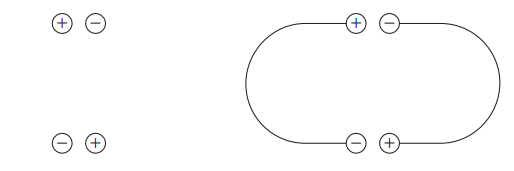
\includegraphics[width=8cm]{Electrodynamics/images/fig3.7-8.PNG}
\end{center}

\begin{proof}
Why will current flow? Well, we have a situation where the \textit{total} charge on each conductor is zero; therefore, there should be a unique way of distributing the charges across each conductor that generate the external electric field. \textit{One} way of doing so involves simply making the charge zero everywhere in each conductor. By the second uniqueness theorem we just proved, this is the \textit{only} way! So the charge will flow along the wires, canceling off.
\end{proof}

\section{The Method of Images}

\subsection{The Classic Image Problem}

It's time to present an incredible trick; it will almost feel like cheating.

\begin{example}
Suppose a point charge $q$ is held a distance $d$ above an infinite grounded conducting plane. What is the potential in the region above the plane?
\end{example}

\begin{proof}
First, note that the answer isn't simply $\frac{1}{4\pi\varepsilon_0}\frac{q}{\scr}$; the conducting plane actually does something since the electric field induces some negative charge on the nearby surface of the conductor, which affects the potential.

But how can we possibly determine the potential, if we don't know how much charge is induced or how it is distributed?

Let's place the infinite grounded conducting plane in the $xy$-plane, and the point charge at $(0,0,d)$ along the $z$-axis. Now, the problem is to solve Poisson's equation in the half-plane $z>0$ with a single point charge $q$ at $(0,0,d)$, subject to the boundary conditions
\begin{enumerate}
    \item $V=0$ when $z=0$ (as the conducting plane is grounded),
    \item $V\to 0$ at infinity.
\end{enumerate}
The first uniqueness theorem guarantees that there is a unique function $V$ that satisfies these boundary conditions. How can we construct such a function?

Here's the trick: consider a completely different setup, which consists of a point charge $q$ at $(0,0,d)$ and a point charge $-q$ at $(0,0,-d)$. The key point is that the half-plane $z>0$ has the same charge distribution, and the boundary conditions still hold:
\begin{enumerate}
    \item $V=0$ when $z=0$,
    \item $V\to 0$ at infinity.
\end{enumerate}
This is because the symmetric placement of a $-q$ charge ensures that the electric potential cancels along $z=0$. Therefore, the solution to $V$ in this setup, by the first uniqueness theorem, \textit{is the same} as the solution to $V$ in the first setup. Hence, the answer is
\[V(x,y,z)=\frac{q}{4\pi\varepsilon_0}\left[\frac{1}{\sqrt{x^2+y^2+(z-d)^2}}-\frac{1}{\sqrt{x^2+y^2+(z+d)^2}}\right] \qquad (z\ge 0).\]
The ``lower region" $z<0$ is still completely different, and we do not understand it using this method.
\end{proof}

\subsection{Induced Surface Charge}

\begin{example}\label{pointconductingplanecharge}
In the setup above, determine the surface charge $\sigma$ induced on the conductor.
\end{example}

\begin{proof}
In the most general situation, we can simply invoke the equation
\[\frac{\partial V}{\partial n}=-\frac{\sigma}{\varepsilon_0}\]
from Subsection \ref{surfcharforcond}, where $\frac{\partial V}{\partial n}=(\nabla V)\cdot\hat{n}$ is the directional derivative in the normal direction.

In the situation above, we can take
\begin{align*}
\sigma(x,y)&=-\varepsilon_0\left.\frac{\partial V}{\partial z}\right\rvert_{z=0}\\
&=-\varepsilon_0\cdot \frac{q}{4\pi\varepsilon_0}\left[\frac{d-z}{(x^2+y^2+(z-d)^2)^{3/2}}+\frac{d+z}{(x^2+y^2+(z+d)^2)^{3/2}}\right]_{z=0}\\
&=\boxed{\frac{-qd}{2\pi(x^2+y^2+d^2)^{3/2}}}.
\end{align*}
For some sanity checks, note that the induced charge is negative and greatest at $x=y=0$. For a further sanity check, we can integrate it over the plane
\begin{align*}
    \iint_{\mathbb{R}^2}\sigma(x,y)da&=\int_{\theta=0}^{2\pi}\int_{r=0}^\infty \frac{-qd}{2\pi(r^2+d^2)^{3/2}}\cdot rdrd\theta\\
    &=-q\int_{0}^\infty\frac{rd}{(r^2+d^2)^{3/2}}dr\\
    &=-q\left[\frac{d}{2}\cdot \frac{-2}{\sqrt{r^2+d^2}}\right]_0^\infty=-q,
\end{align*}
as expected.

\end{proof}

\subsection{Force and Energy}

\begin{example}
What is the force of attraction between the point charge and the plane?
\end{example}

\begin{proof}
Once again, considering the analog problem with two point charges $+q$ and $-q$ suffices, since the local potential around $+q$ is all that determines the force on it, and it is the same in both setups. Therefore, the force is simply
\[\vec{F}=-\frac{1}{4\pi\varepsilon_0}\frac{q^2}{(2d)^2}\hat{z}.\]
\end{proof}

\begin{example}
How do the energies of the two analogous setups (the point charge and plane versus the two opposite point charges) compare?
\end{example}

\begin{proof}
With two point charges, the energy is simply
\[W=-\frac{1}{4\pi\varepsilon_0}\frac{q^2}{2d}.\]
However, it turns out that for a single charge and conducting plane, the energy is \textit{half}:
\[W=-\frac{1}{4\pi\varepsilon_0}\frac{q^2}{4d}.\]
One way to figure out why is to consider the energy stored in the fields
\[W=\iiint_{\mathbb{R}^3}\frac{\varepsilon_0E^2}{2}d\tau,\]
and note that in the plane case we only have the upper region $z\ge 0$ of fields, so we should only get half the energy.

We can also compute the energy by calculating the work required to bring $q$ in from infinity.
\end{proof}

\begin{remark}
One way to conceptualize the difference between these cases is that with the plane,w e are doing work on a \textit{single} point charge to bring it in. The induced charge on the conductor is shifting around, but this costs no work since the potential is zero (you can also think of the fact that it is a conductor, so charge can move around freely).

In the analog case with two charges, however, we need to do work to pull in \textit{both} of them, so the energy stored is twice as much.
\end{remark}

\subsection{Other Image Problems}

We can apply the above technique to any collection of point charges near a grounded conducting plane by introducing the mirror image of the setup with opposite charges (notice how introducing these opposite charges ensures that the potential along where the plane should be is 0). We call this the \vocab{method of images}.

The following application of the method of images is beautiful, and relates to circle (sphere) inversion and Apollonius circles (spheres).

\begin{example}
A point charge $q$ is situated a distance $a$ from the center of a grounded conducting sphere of radius $R$. Find the potential outside the sphere.
\end{example}

\begin{proof}
\textit{Invert} (!!) the point charge $q$ about the sphere; this gives a point that is a distance 
\[b=\frac{R^2}{a}\]
away from the center, along the ray from the center of the sphere to the point charge $q$. Imbue this point charge with charge
\[q'=-\frac{R}{a}q.\]
We claim that this setup has zero potential along the surface of the sphere; this is true by Appolonius spheres. Therefore, the potential is indeed
\[\boxed{V(\vec{r})=\frac{1}{4\pi\varepsilon_0}\left(\frac{q}{\scr}+\frac{q'}{\scr'}\right)}\]
outside the sphere, where $\scr$ is the distance to $q$ and $\scr'$ is the distance to $q'$.
\end{proof}

\begin{remark}
You cannot place image charges in the region where you are calculating $V$! That would charge $\rho$, and you'd be solving Poisson's equation with incorrect $\rho$ (even if the boundary conditions are the same).
\end{remark}

\begin{example}
What is the force of attraction between the point and sphere?
\end{example}

\begin{proof}
It is simply the force between the charge and the image charge $q'$ we placed:
\[F=\frac{1}{4\pi\varepsilon_0}\frac{qq'}{(a-b)^2}=\boxed{-\frac{1}{4\pi\varepsilon_0}\frac{q^2Ra}{(a^2-R^2)^2}}.\]
\end{proof}

The method of images is incredibly simple and magical. It comes down to figuring out the correct ``auxiliary" configuration of image charges to make sure the grounded conductors in the setup have potential zero. However, for most shapes, this is forbiddingly complicated, if not impossible. So use with care!

\section{Separation of Variables}

Recall that in Section \ref{boundconduniqthm} we proved the first uniqueness theorem, which states that if $V$ is given on a boundary $\partial\mathcal{V}$, then it is uniquely determined on the interior of the volume, and therefore the entire volume $\mathcal{V}$. This is because $V$ satisfies Laplace's equation $\nabla^2 V=0$ (assuming there is no charge distribution in the volume).

In this section, we try to solve this problem exactly, mathematically. We use a technique called \vocab{separation of variables}. We'll develop the method through a sequence of examples in various coordinate systems.

\subsection{Cartesian Coordinates}

\begin{example}
Two infinite grounded metal plates lie parallel to the $xz$ plane, one at $y=0$, the other at $y=a$. The left end, at $x=0$, is closed off with an infinite strip insulated from the two plates, and maintained at a specific potential $V_0(y)$. Find the potential inside this ``slot."
\end{example}

\begin{center}
    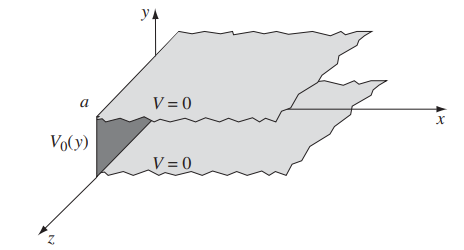
\includegraphics[width=8cm]{Electrodynamics/images/fig3.17.PNG}
\end{center}

\begin{remark}
For an actual physical example of how such a situation could occur, consider placing an infinite charged wire parallel to the $z$ axis at $y=a/2$ and $x=0$, between the two parallel grounded metal plates. This generates some potential along the infinite strip along the $yz$ plane. It also generates some potential in the rest of the volume, but this is the point: our goal is to compute the potential in the slot given the potential along the boundary.
\end{remark}

\begin{proof}
Our goal is to use Laplace's equation $\nabla^2V=0$ to get $V$ in the interior. Note that $V_0(y)$ doesn't depend on $z$, so this is really a $2$-dimensional problem:
\[\frac{\partial^2V}{\partial x^2}+\frac{\partial^2V}{\partial y^2}=0.\]
We are subject to the following boundary conditions:
\begin{enumerate}[(i)]
    \item $V=0$ when $y=0$,
    \item $V=0$ when $y=a$,
    \item $V=V_0(y)$ when $x=0$,
    \item $V\to 0$ when $x\to\infty$.
\end{enumerate}
Since we have $V$ on all the boundaries, by the first uniqueness theorem, it should be uniquely determined within the slot.

Here's the leap: we will start by only investigating solutions $V(x,y)$ to $\nabla^2V=0$ such that it can be expressed as a product of a function depending \textit{only} on $x$ and a function depending \textit{only} on $y$:
\[V(x,y)=X(x)Y(y).\]
This is an \textit{absurd} restriction; we cannot expect $V$ to actually satisfy this! Even something as simple as $V(x,y)=5x+6y$ cannot be written in this form.

However, it turns out that magically, the solutions we \textit{do} get are very special, and pasting them together through linear combinations allows us to construct the general solution. After all, if functions $V_i$ satisfy $\nabla^2 V_i=0$ for all $i$ then so do any linear combinations:
\[\nabla^2\left(\sum_ic_iV_i\right)=\sum_{i}c_i\nabla^2(V_i)=0.\]

Plugging $V(x,y)=X(x)Y(y)$ into $\nabla^2 V=0$ gives
\[\frac{d^2X}{dx^2}Y+X\frac{d^2Y}{dy^2}=0\implies \frac{1}{X}\frac{d^2X}{dx^2}+\frac{1}{Y}\frac{d^2Y}{dy^2}=0.\]
Since these terms are independent (one depends only on $x$ and the other depends only on $y$), they must both be constant. Due to the boundary conditions (this will be clear later), we require that $\frac{1}{X}\frac{d^2X}{dx^2}$ be the positive term. Therefore, we can let
\[\frac{d^2X}{dx^2}=k^2X, \qquad \frac{d^2Y}{dy^2}=k^2Y.\]
These are easy to solve by standard ordinary differential equations methods:
\[X(x)=Ae^{kx}+Be^{-kx}, \qquad Y(y)=C\sin(ky)+D\cos(ky).\]
Hence,
\[V(x,y)=(Ae^{kx}+Be^{-kx})(C\sin(ky)+D\cos(ky)).\]
Now, we need to satisfy the boundary conditions. Boundary condition (iv) requires that $A=0$. Further, boundary condition (i) requires that $D=0$. Finally, (ii) requires that $\sin(ka)=0\implies k=\frac{n\pi}{a}$ for $n\in \NN$. 

That is as far as we can go; unless $V_0(y)$ is some multiple of $\sin\left(\frac{n\pi y}{a}\right)$, we cannot simply fit to (iii). However, it turns out that we can use linear combinations to do so. Patching together our separable solutions allows us to construct much more general functions:
\[V(x,y)=\sum_{n=1}^\infty C_ne^{-n\pi x/a}\sin(n \pi y/a).\]
Now, the goal is to fit
\[V_0(y)=V(0,y)=\sum_{n=1}^\infty C_n\sin(n\pi y/a).\]
This is a \vocab{Fourier sine series}, which by Dirichlet's theorem, is guaranteed to be able to match virtually \textit{any} function $V_0(y)$---even if it has a finite number of discontinuities.

To determine the coefficients, we can use \vocab{Fourier's trick} (which Euler seems to have developed earlier):
\[\int_0^aV_0(y)\sin(n'\pi y/a)dy=\sum_{n=1}^\infty C_n\int_0^a\sin(n\pi y/a)\sin(n'\pi y/a)dy.\]
Now, we can compute that
\[\int_0^a \sin(n\pi y/a)\sin (n'\pi y/a)dy=\begin{cases}
0, & \text{if }n'\neq n,\\
\frac{a}{2}, & \text{if }n'=n.
\end{cases}\]
Hence, extracting the coefficients just amounts to
\[C_n=\frac{2}{a}\int_0^aV_0(y)\sin(n\pi y/a)dy.\]
And we are done:
\[\boxed{V(x,y)=\frac{2}{a}\sum_{n=1}^\infty \left(\int_0^a V_0(y)\sin(n\pi y/a)dy\right)e^{-n\pi x/a}\sin(n\pi y/a)}.\]
\end{proof}

\begin{remark}\label{fixedpot}
For a concrete example, suppose $V_0(y)=V_0$ is a fixed potential. Then,
\[C_n=\frac{2V_0}{a}\int_0^a\sin(n\pi y/a)dy=\frac{2V_0}{n\pi}(1-\cos(n\pi))=\begin{cases}
0, & \text{if }2\mid n,\\
\frac{4V_0}{n\pi} & \text{otherwise}.
\end{cases}\]
Hence, 
\[V(x,y)=\frac{4V_0}{\pi}\sum_{n\text{ odd}}\frac{1}{n}e^{-n\pi x/a}\sin(n\pi y/a)=\frac{2V_0}{\pi}\tan^{-1}\left(\frac{\sin(\pi y/a)}{\sinh (\pi x/a)}\right).\]
Below is a picture of such a potential.
\end{remark}

\begin{center}
    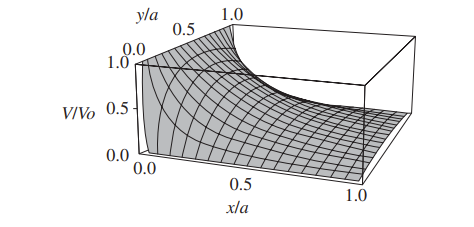
\includegraphics[width=8cm]{Electrodynamics/images/fig3.18.PNG}
\end{center}

This technique is very beautiful, and the mathematics behind it underlines the \vocab{Fourier transform}. If you know some linear algebra, there's a pretty nice way to understand what just happened.

We can consider the vector space of all functions on the interval $[0,a]$; then, we equip the space with an inner product given by
\[\langle f,g\rangle = \frac{2}{a}\int_0^af(y)\ol{g(y)}\cdot dy.\]
However, since $f,g$ are real functions, the complex conjugate doesn't matter. It turns out that this turns the vector space into a \vocab{Hilbert space}; the distance function
\[||f-g||=\sqrt{\langle f-g, f-g\rangle}\]
defined by the inner product makes it a complete metric space (all Cauchy sequences converge). You can check that $||f-g||$ behaves as your intuition would suggest (and therefore our inner product is a good choice): if $f$ and $g$ don't differ much, then $\langle f-g,f-g\rangle$ is small. Now, here's the big claim:

\begin{claim}
The set of functions 
\[\mathcal{B}=\left\{e_n:=\sin\left(\frac{n\pi y}{a}\right):n\in \NN\right\}\]
forms an orthonormal basis of this Hilbert space.
\end{claim}

\begin{proof}
The main point is checking orthogonality: we can do so by just taking inner products:
\begin{align*}
\langle e_m,e_n\rangle &= \frac{2}{a}\int_0^a \sin\left(\frac{m\pi y}{a}\right)\sin\left(\frac{n\pi y}{a}\right)dy\\
&=\frac{1}{a}\int_0^a\left[\cos\left(\frac{(m-n)\pi y}{a}\right)-\cos\left(\frac{(m+n)\pi y}{a}\right)\right]dy=0
\end{align*}
when $m\neq n$. However, if $m=n$, we instead have that it is equal to $1$.

Therefore, $\mathcal{B}$ are indeed orthonormal. Checking that they are spanning as a basis is harder and outside the scope of this text.
\end{proof}

Now, the motivation for Fourier's trick is very clear. If we express any function $f$ in $[0,a]^*$ as a linear combination of vectors in $\mathcal{B}$, we get
\[f=\sum_{n=1}^\infty c_ne_n.\]
Yet in linear algebra, if we ever have a vector written as a linear combination of orthonormal basis vectors in a vector space, how do we extract the coefficients $c_n$? Well, we take the inner product of $f$ with a given basis vector $e_{n'}$:
\begin{align*}
\langle f,e_{n'}\rangle&=\left\langle \sum_{n=1}^\infty c_ne_n, e_{n'}\right\rangle\\
&=\sum_{n=1}^\infty c_n\langle e_n, e_{n'}\rangle\\
&=c_n,
\end{align*}
by linearity of the inner product and the fact that $\langle e_n, e_{n'}\rangle$ equals $0$ when $n\neq n'$ and $1$ when $n=n'$ (orthonormal basis). Therefore,
\[c_n=\langle f,e_n\rangle = \frac{2}{a}\int_0^af(y)\sin(n\pi y/a)dy,\]
as shown before.

\begin{remark}
This linear algebra is really the same computations as the proof of the theorem, but I just find it a nicer way to frame the whole Fourier transform argument.
\end{remark}

Let's do some more examples!

\begin{example}
Two infinitely-long grounded metal plates, again at $y = 0$ and $y = a$, are connected at $x = \pm b$ by metal strips maintained at a constant potential $V_0$, as shown below (a thin layer of insulation at each corner prevents them from shorting out). Find the potential inside the resulting rectangular pipe.
\end{example}

\begin{center}
    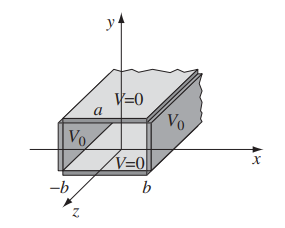
\includegraphics[width=8cm]{Electrodynamics/images/fig3.20.PNG}
\end{center}

\begin{proof}
Once again, the setup doesn't depend on the $z$-coordinate, so it's really a 2-dimensional problem
\[\frac{\partial^2V}{\partial x^2}+\frac{\partial^2V}{\partial y^2}=0\]
under boundary conditions
\begin{enumerate}[(i)]
    \item $V=0$ when $y=0$,
    \item $V=0$ when $y=a$,
    \item $V=V_0$ when $x=-b$,
    \item $V=V_0$ when $x=+b$.
\end{enumerate}
Once again, we search for \textit{separable} functions
\[V(x,y)=X(x)Y(y)\implies \frac{1}{X}\frac{d^2X}{dx^2}+\frac{1}{Y}\frac{d^2Y}{dy^2}=0.\]
Once again, both these terms must be constant:
\[\frac{d^2X}{dx^2}=k^2X, \qquad \frac{d^2Y}{dy^2}=-k^2Y.\]
Solving gives
\[X(x)=Ae^{kx}+Be^{-kx}, \qquad Y(y)=C\sin(kx)+D\cos(kx).\]
Since $V(x,y)=V(-x,y)$, we have $A=B$, so we can write
\[V(x,y)=\cosh (kx)(C\sin (ky)+D\cos (ky)).\]
Further, boundary conditions (i) and (ii) gives $D=0$ and $k=n\pi /a$. Thus,
\[V(x,y)=C\cosh(n\pi x/a)\sin(n\pi y/a).\]
Now, we need to match boundary condition (iii) (note that (iv) follows immediately from the even-ness in $x$).

To do so, let's use a linear combination
\[V(x,y)=\sum_{n=1}^\infty C_n
\cosh(n\pi x/a)\sin(n\pi y/a).\]
Now, we require that
\[V_0=V(b,y)=\sum_{n=1}^\infty \left(C_n\cosh (n\pi b/a)\right)\sin(n\pi y/a).\]
From Remark \ref{fixedpot}, this implies
\[C_n\cosh(n\pi b/a)=\begin{cases}
0, & \text{if }2\mid n,\\
1, & \text{otherwise}.
\end{cases}\]
Finally, the potential in this case is
\[\boxed{V(x,y)=\frac{4V_0}{\pi}\sum_{n\text{ odd}}\frac{1}{n}\frac{\cosh(n\pi x/a)}{\cosh(n\pi b/a)}\sin(n\pi y/a)}\]
\end{proof}

\begin{example}
An infinitely long rectangular metal pipe (sides $a$ and $b$) is grounded, but one end, at $x = 0$, is maintained at a specified potential $V_0(y,z)$, as indicated in the figure below. Find the potential inside the pipe.
\end{example}

\begin{center}
    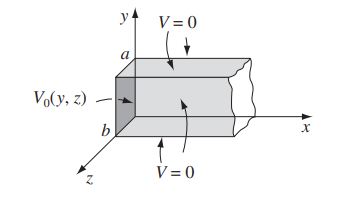
\includegraphics[width=8cm]{Electrodynamics/images/fig3.22.PNG}
\end{center}

\begin{proof}
Now we have a truly three-dimensional problem. We need to solve
\[\frac{\partial^2V}{\partial x}+\frac{\partial^2V}{\partial y}+\frac{\partial^2V}{\partial z}=0\]
under boundary conditions
\begin{enumerate}[(i)]
    \item $V=0$ when $y=0$ or $y=a$,
    \item $V=0$ when $z=0$ or $z=b$,
    \item $V\to 0$ when $x\to \infty$,
    \item $V=V_0(y,z)$ when $x=0$.
\end{enumerate}
As before, we consider separable $V(x,y,z)=X(x)Y(y)Z(z)$ and note that
\[\frac{1}{X}\frac{d^2X}{dx^2}+\frac{1}{Y}\frac{d^2Y}{dy^2}+\frac{1}{Z}\frac{d^2Z}{dz^2}=0.\]
From our previous experience, we should let
\[\frac{d^2X}{dx^2}=(k^2+\ell^2)X, \qquad \frac{d^2Y}{dy^2}=-k^2Y, \qquad \frac{d^2Z}{dz^2}=-\ell^2Z.\]
Solving these differential equations and applying boundary conditions (i) through (ii) gives
\[V(x,y,z)=Ce^{-\pi\sqrt{(n/a)^2+(m/b)^2}x}\sin(n\pi y/a)\sin(m\pi z/b),\]
where we set $k=n\pi/a$ and $\ell=m\pi/b$. Now, we can construct linear combinations which are still solutions to $\nabla^2V=0$:
\[V(x,y,z)=\sum_{n=1}^\infty \sum_{m=1}^\infty C_{n,m}e^{-\pi\sqrt{(n/a)^2+(m/b)^2}x}\sin(n\pi y/a)\sin(m\pi z/b).\]
For the final boundary condition, we need
\[V_0(y,z)=V(0,y,z)=\sum_{n=1}^\infty \sum_{m=1}^\infty C_{n,m}\sin(n\pi y/a)\sin(m\pi z/b).\]
To solve this, we can just use Fourier's trick twice:
\begin{align*}
\int_0^a\int_0^b&V_0(y,z)\sin(n'\pi y/a)\sin(m'\pi z/b)dzdy\\
&=\sum_{n=1}^\infty\sum_{m=1}^\infty C_{n,m}\int_0^a\sin(n\pi y/a)\sin(n'\pi y/a)dy\int_0^b\sin(m\pi z/b)\sin(m'\pi z/b)dz\\
&=\frac{ab}{4}C_{n',m'}.
\end{align*}
Hence, 
\[C_{n,m}=\frac{4}{ab}\int_0^a\int_0^bV_0(y,z)\sin(n\pi y/a)\sin(m\pi z/b)dzdy.\]
Plugging this in gives a general solution of
\begin{empheq}[box=\fbox]{align*}
  V(x,y,z)=&\sum_{n=1}^\infty \sum_{m=1}^\infty \left[\frac{4}{ab}\int_0^a\int_0^bV_0(y,z)\sin(n\pi y/a)\sin(m\pi z/b)dzdy\right]\\
  &\cdot e^{-\pi\sqrt{(n/a)^2+(m/b)^2}x}\sin(n\pi y/a)\sin(m\pi z/b).
\end{empheq}
\end{proof}

\subsection{Spherical Coordinates}

In the examples we've seen so far, the boundaries have been planes. However, for round objects, spherical coordinates are more natural. In this coordinate system, Laplace's equation reads
\[\frac{1}{r^2}\frac{\partial}{\partial r}\left(r^2\frac{\partial V}{\partial r}\right)+\frac{1}{r^2\sin\theta}\frac{\partial}{\partial\theta}\left(\sin\theta\frac{\partial V}{\partial\theta}\right)
+\frac{1}{r^2\sin^2\theta}\frac{\partial^2V}{\partial \varphi^2}=0.\]
In the scope of this book, we will only consider problems with \vocab{azimuthal symmetry}, which means that $V$ is independent of $\varphi$. Then, the equation reduces to
\[\frac{\partial}{\partial r}\left(r^2\frac{\partial V}{\partial r}\right)+\frac{1}{\sin\theta}\frac{\partial}{\partial \theta}\left(\sin\theta\frac{\partial V}{\partial \theta}\right)=0.\]
Once again, we only consider solutions that are products:
\[V(r,\theta)=R(r)\Theta(\theta).\]
Plugging this in and dividing by $R\Theta$ gives
\[\frac{1}{R}\frac{d}{dr}\left(r^2\frac{dR}{dr}\right)+\frac{1}{\Theta\sin\theta}\frac{d}{d\theta}\left(\sin\theta\frac{d\Theta}{d\theta}\right)=0.\]
Both of these must be constant. For aesthetic reasons later (the differential equations will have solutions in nicer forms), we write this constant in the form $\ell(\ell+1)$:
\[\frac{1}{R}\frac{d}{dr}\left(r^2\frac{dR}{dr}\right)=\ell(\ell+1), \qquad \frac{1}{\Theta\sin\theta}\frac{d}{d\theta}\left(\sin\theta\frac{d\Theta}{d\theta}\right)=-\ell(\ell+1).\]
It turns out the solution to the radial equation is simply
\[R(r)=Ar^\ell+\frac{B}{r^{\ell+1}},\]
which can be easily checked (we expect two free variables $A$ and $B$ from this ordinary second-order differential equation). The angular equation, however, is not so simple: the solutions are given by the following polynomials:
\begin{definition}
The solutions to the angular equation are (multiples of) \vocab{Legendre polynomials} in the variable cosine:
\[\Theta(\theta)=P_\ell(\cos\theta),\]
where $P_\ell$ is given by \vocab{Rodrigues formula}
\[P_\ell(x):=\frac{1}{2^\ell \ell!}\frac{d^\ell}{dx^\ell}(x^2-1)^\ell.\]
\end{definition}
\begin{remark}
We expect two linearly independent solutions (and to be able to take linear combinations of these solutions) for this second-order differential equation, but it turns out these other solutions blow up at either $\theta=0$ or $\theta=\pi$, and are therefore unacceptable on physical grounds. (In rare cases where the $z$-axis is excluded, these other solutions do have to be considered.)

For example, the second solution for $\ell=0$ is
\[\Theta(\theta)=\ln\left(\tan\frac{\theta}{2}\right).\]
\end{remark}

\begin{example}[Some Legendre polynomials]\label{somelegpoly}
For small values of $\ell$, we have
\begin{itemize}
    \item $P_0(x)=1$,
    \item $P_1(x)=x$,
    \item $P_2(x)=(3x^2-1)/2$,
    \item $P_3(x)=(5x^3-3x)/2$,
    \item $P_4(x)=(35x^4-30x^2+3)/8$,
    \item $P_5(x)=(63x^5-70x^3+15x)/8$.
\end{itemize}

Note that $P_\ell(x)$ has degree $\ell$; in addition, the constant out front is chosen so that $P_\ell(1)=1$.
\end{example}

Therefore, the most general physical separable solutions to Laplace's equation are given by
\[V(r,\theta)=\left(Ar^\ell+\frac{B}{r^{\ell+1}}\right)P_\ell(\cos\theta).\]
We can use linear combinations to generate an even more general solution:
\[\boxed{V(r,\theta)=\sum_{\ell=0}^\infty \left(A_\ell r^\ell+\frac{B_\ell}{r^{\ell+1}}\right)P_\ell(\cos\theta)}.\]
Let's demonstrate the power of this result through a sequence of examples:

\begin{example}
The potential $V_0(\theta)$ is specified on the surface of a hollow sphere, of radius $R$. Find the potential inside the sphere.
\end{example}

\begin{proof}
This is a clear example of the second uniqueness theorem: we're given $V$ on the boundary of a sphere and are trying to compute it inside the surface.

In the boxed equation above, we clearly have $B_\ell=0$ for all $\ell$, since otherwise the potential would blow up at the origin. Thus
\[V(r,\theta)=\sum_{\ell=0}^\infty A_\ell r^\ell P_\ell(\cos\theta).\]
Now, we need to match
\[V_0(\theta)=V(R,\theta)=\sum_{\ell=0}^\infty A_\ell R^\ell P_\ell(\cos\theta).\]
As it turns out, Legendre polynomials (like the sine functions), constitute a \textit{complete} and \textit{orthogonal} set of functions for $-1\le x\le 1$ (so $0\le \theta\le \pi$). Hence, they form an orthogonal basis (depending on the definition of the norm and scaling the functions, you can get a orthonormal basis).

In any case, Fourier's trick works since
\[\int_{-1}^1P_\ell(x)P_{\ell'}(x)dx = \int_0^\pi P_\ell(\cos\theta)P_{\ell'}(\cos\theta)\sin\theta d\theta=\begin{cases}
0 & \text{if } \ell'\neq \ell,\\
\frac{2}{2\ell+1} & \text{if }\ell'=\ell.
\end{cases}\]
Therefore, in order to extract the coefficient $A_{\ell'}$, it suffices to multiply by $P_{\ell'}(\cos\theta)\sin\theta$ and integrate:
\[\int_0^\pi V_0(\theta)P_{\ell'}(\cos\theta)\sin\theta d\theta = \sum_{\ell=0}^\infty A_\ell r^\ell\int_0^\pi P_{\ell}(\cos\theta)P_{\ell'}(\cos\theta)\sin\theta d\theta = A_{\ell'}R^{\ell'}\cdot \frac{2}{2\ell'+1}.\]
Hence,
\[A_\ell=\frac{2\ell+1}{2R^\ell}\int_0^\pi V_0(\theta)P_{\ell}(\cos\theta)\sin\theta d\theta.\]
Plugging this in gives a general solution of
\[\boxed{V(r,\theta)=\sum_{\ell=1}^\infty \left[\frac{2\ell+1}{2R^\ell}\int_0^\pi V_0(\theta)P_{\ell}(\cos\theta)\sin\theta d\theta\right]\cdot r^\ell P_\ell(\cos\theta)}.\]
\end{proof}

\begin{remark}
Often, the integral
\[A_\ell=\frac{2\ell+1}{2R^\ell}\int_0^\pi V_0(\theta)P_{\ell}(\cos\theta)\sin\theta d\theta\]
can be hard to compute, so in practice it's often easier to solve
\[V_0(\theta)=\sum_{\ell=0}^\infty A_{\ell}r^\ell P_\ell(\cos\theta)\]
by eye, leveraging Example \ref{somelegpoly}. For instance, if the potential on the sphere is $V_0(\theta)=k\sin^2(\theta/2)$,
then we can rewrite it as
\[V_0(\theta)=\frac{k}{2}(1-\cos\theta)=\frac{k}{2}[P_0(\cos\theta)-P_1(\cos\theta)],\]
giving
\[V(r,\theta)=\frac{k}{2}\left[P_0(\cos\theta)-\frac{r}{R}P_1(\cos\theta)\right]=\frac{k}{2}\left(1-\frac{r}{R}\cos\theta\right).\]
\end{remark}

\begin{example}
The potential $V_0(\theta)$ is again specified on the surface of a sphere of radius $R$, but this time we are asked to find the potential \textit{outside}, assuming there is no charge there.
\end{example}

\begin{proof}
This time, we need $A_\ell=0$ for all $\ell$, otherwise $V$ wouldn't be zero at $r\to\infty$. Thus,
\[V(r,\theta)=\sum_{\ell=0}^\infty \frac{B_\ell}{r^{\ell+1}}P_\ell(\cos\theta).\]
This time, for the boundary condition, we need
\[V_0(\theta)=V(R,\theta)=\sum_{\ell=0}^\infty \frac{B_\ell}{R^{\ell+1}}P_\ell(\cos\theta).\]
We can extract coefficients with Fourier's trick again (as the Legendre polynomials are orthogonal), to get
\[B_\ell=\frac{2\ell+1}{2}R^{\ell+1}\int_0^\pi V_0(\theta)P_{\ell}(\cos\theta)\sin\theta d\theta.\]
Plugging this in gives
\[\boxed{V(r,\theta)=\sum_{\ell=0}^\infty \left[\frac{2\ell+1}{2}R^{\ell+1}\int_0^\pi V_0(\theta)P_{\ell}(\cos\theta)\sin\theta d\theta\right]\frac{1}{r^{\ell+1}}P_\ell(\cos\theta)}.\]


\end{proof}

\begin{example}\label{sphereinfield}
An uncharged metal sphere of radius $R$ is placed in an otherwise uniform electric field $\vec{E}=E_0\hat{z}$. The field will push positive charge to the ``northern" surface of the sphere, and---symmetrically---negative charge to the ``southern" surface. This induced charge, in turn, distorts the field in the neighborhood of the plane. Find the potential in the region outside the sphere.
\end{example}

\begin{proof}
Since the entire sphere is an equipotential, we will set it to $V(R,\theta)=0$. Note that the normal convention of $V=0$ at $r\to\infty$ doesn't make sense since we have an electric field that reaches infinitely far (so the potential difference from infinity will be infinite).

Now, we have boundary conditions
\begin{enumerate}[(i)]
    \item $V(R,\theta)=0$,
    \item $V(r,\theta)=-E_0r\cos\theta$ when $r\gg R$.
\end{enumerate}
Recall our general solution
\[V(r,\theta)=\sum_{\ell=0}^\infty\left(A_\ell r^\ell+\frac{B_\ell}{r^{\ell+1}}\right)P_\ell(\cos\theta).\]
Since boundary condition (i) holds for all angles $\theta$, we must have
\[A_\ell R^\ell+\frac{B_\ell}{R^{\ell+1}}=0\]
for all $\ell$ (you can also check this explicitly with Fourier's trick).

Hence, we can write
\[B_\ell=-A_\ell\cdot R^{2\ell+1}.\]
Hence,
\begin{align*}
V(r,\theta)&=\sum_{\ell=0}^\infty\left(A_\ell r^\ell-\frac{A_\ell\cdot R^{2\ell+1}}{r^{\ell+1}}\right)P_\ell(\cos\theta)\\
&=\sum_{\ell=0}^\infty A_\ell r^\ell P_\ell(\cos\theta)\left[1-\left(\frac{R}{r}\right)^{2\ell+1}\right].
\end{align*}
Now we see how to use the condition $r\gg R$ in boundary condition (ii): in this case, we have that $1-(R/r)^{2\ell+1}\to 1$, so
\[-E_0r\cos\theta=V(r,\theta)=\sum_{\ell=0}^\infty A_\ell r^\ell P_\ell(\cos\theta)\qquad(r\gg R).\]
We could now extract the coefficients $A_\ell$ using Fourier's trick, but it's easier to just do by eye:
\[-E_0r\cos\theta=A_0+A_1r\cos\theta+A_2r^2\cdot\frac{3\cos^2\theta-1}{2}+\cdots.\]
Evidently setting $A_1=-E_0$ as the only nonzero coefficient suffices. Hence, the answer is
\[\boxed{V(r,\theta)=-E_0r\left(1-\frac{R^3}{r^3}\right)\cos\theta}.\]
\end{proof}

\begin{remark}
If you were interested in the induced charge density of the sphere:
\[\sigma(\theta)=-\varepsilon_0\left.\frac{\partial V}{\partial r}\right\rvert_{r=R}=\varepsilon_0E_0\left.\left(1+2\frac{R^3}{r^3}\right)\cos\theta\right\rvert_{r=R}=3\varepsilon_0E_0\cos\theta.\]
As expected, the northern hemisphere $\theta\in[0,\pi/2]$ is positively charged and the southern hemisphere $\theta\in[\pi/2,\pi]$ is negatively charged.
\end{remark}

\begin{example}\label{chargespherepotential}
A specified charge density $\sigma_0(\theta)$ is glued over the surface of a spherical shell of radius $R$. Find the resulting potential inside and outside the sphere.
\end{example}

\begin{proof}
In theory, you could do this by just directly integrating:
\[V=\frac{1}{4\pi\varepsilon_0}\iint_{\mathcal{S}}\frac{\sigma_0}{\scr}da,\]
but separation of variables is often an easier technique.

For the potential inside, once again we need $B_\ell=0$ for all $\ell$ otherwise the potential at the origin would blow up:
\[V(r,\theta)=\sum_{\ell=0}^\infty A_\ell r^\ell P_\ell(\cos\theta)\qquad (r\le R),\]
while for the potential outside, we need $A_\ell=0$ for all $\ell$ otherwise the potential at infinity would blow up:
\[V(r,\theta)=\sum_{\ell=0}^\infty \frac{B_{\ell}}{r^{\ell+1}}P_\ell(\cos\theta)\qquad (r\ge R).\]
First of all, we need these to agree at the boundary $r=R$:
\[\sum_{\ell=0}^\infty A_\ell R^\ell P_\ell(\cos\theta)=V(R,\theta)=\sum_{\ell=0}^\infty \frac{B_\ell}{R^{\ell+1}}P_\ell(\cos\theta).\]
As this applies for \textit{any} angle $\theta$ (and the Legendre polynomials are linearly independent), we require that
\[A_\ell R^\ell=\frac{B_\ell}{R^{\ell+1}}\implies B_\ell=A_\ell R^{2\ell+1}\]
for every $\ell$. We can also get this result using Fourier's trick:
\begin{align*}
\int_0^\pi \left(\sum_{\ell=0}^\infty A_\ell R^\ell P_\ell(\cos\theta)\right)P_{\ell'}(\cos\theta)\sin\theta d\theta &= \int_0^\pi\left(\sum_{\ell=0}^\infty \frac{B_\ell}{R^{\ell+1}}P_\ell(\cos\theta)\right)P_{\ell'}(\cos\theta)\\
\sum_{\ell=0}^\infty A_\ell R^\ell \left[\int_0^\pi P_\ell(\cos\theta)P_{\ell'}(\cos\theta)\sin\theta d\theta\right]&=\sum_{\ell=0}^\infty \frac{B_\ell}{R^{\ell+1}}\left[\int_0^\pi P_{\ell}(\cos\theta)P_{\ell'}(\cos\theta)\sin\theta d\theta\right]\\
A_{\ell'}R^{\ell'}\cdot\frac{2}{2\ell'+1}&=\frac{B_{\ell'}}{R^{\ell'+1}}\cdot \frac{2}{2\ell'+1}.
\end{align*}
Therefore, we can write the potential outside as
\[V(r,\theta)=\sum_{\ell=0}^\infty A_\ell r^\ell P_\ell(\cos\theta)\cdot \left(\frac{R}{r}\right)^{2\ell+1}\qquad (r\ge R).\]

Now, recall that the surface charge density tells us the difference in the directional derivative of $V$ in the direction of the normal to the surface:
\[-\frac{\sigma}{\varepsilon_0}=\left.\frac{\partial V}{\partial r}\right\rvert_{r\to R^+}-\left.\frac{\partial V}{\partial r}\right\rvert_{r\to R^-}.\]
For $r\to R^-$, we can compute the derivative of the equation for $r\le R$:
\[\frac{\partial V(r,\theta)}{\partial r}=\frac{\partial}{\partial r}\left[\sum_{\ell=0}^\infty A_\ell r^\ell P_\ell(\cos\theta)\right]=\sum_{\ell=1}^\infty \ell A_\ell r^{\ell-1}P_\ell(\cos\theta)\qquad (r\le R).\]
Similarly, for $r\to R^+$, we can compute the derivative of the equation for $r\ge R$:
\[\frac{\partial V(r,\theta)}{\partial r}=\left[\frac{\partial}{\partial r}\sum_{\ell=0}^\infty A_{\ell} r^\ell P_\ell(\cos\theta)\cdot\left(\frac{R}{r}\right)^{2\ell+1}\right]=\sum_{\ell=0}^\infty -(\ell+1)A_\ell \cdot \frac{R^{2\ell+1}}{r^{\ell+2}}P_\ell(\cos\theta).\]
When $r=R$, we have
\[-\frac{\sigma_0(\theta)}{\varepsilon_0}=\sum_{\ell=0}^\infty -(2\ell+1)A_\ell R^{\ell-1}P_\ell(\cos\theta).\]
At this point, the coefficients can be extracted using Fourier's trick:
\[\frac{1}{\varepsilon_0}\int_0^\pi \sigma_0(\theta)P_{\ell'}(\cos\theta)\sin\theta d\theta=(2\ell'+1)A_{\ell'}R^{\ell'-1}\cdot \frac{2}{2\ell'+1},\]
so
\[A_{\ell}=\frac{1}{2\varepsilon_0 R^{\ell-1}}\int_0^\pi \sigma_0(\theta)P_\ell(\cos\theta)\sin\theta d\theta.\]
Therefore, the full solution is
\[\boxed{V(r,\theta)=\begin{dcases}
\sum_{\ell=0}^\infty \left[\frac{1}{2\varepsilon_0 R^{\ell-1}}\int_0^\pi \sigma_0(\theta)P_\ell(\cos\theta)\sin\theta d\theta\right]r^\ell P_\ell(\cos\theta) & \text{if }r\le R,\\
\sum_{\ell=0}^\infty \left[\frac{1}{2\varepsilon_0 R^{\ell-1}}\int_0^\pi \sigma_0(\theta)P_\ell(\cos\theta)\sin\theta d\theta\right]r^\ell P_\ell(\cos\theta)\cdot\left(\frac{R}{r}\right)^{2\ell+1} & \text{if }r\ge R.
\end{dcases}}\]
\end{proof}

\begin{remark}
As a concrete example, suppose $\sigma_0(\theta)=k\cos\theta=kP_1(\cos\theta)$; then, the only nonzero $A_\ell$ is clearly $\ell=1$, equal to
\[A_1=\frac{k}{3\varepsilon_0}.\]
Thus, inside the sphere we have
\[V(r,\theta)=\frac{kr}{3\varepsilon_0}\cos\theta \qquad (r\le R),\]
while outside we have
\[V(r,\theta)=\frac{kR^3}{3\varepsilon_0r^2}\cos\theta\qquad (r\ge R).\]
In particular, in the situation of Example \ref{sphereinfield}, the surface charge is $\sigma_0(\theta)=3\varepsilon_0 E\cos\theta$, so the potential inside is
\[V(r,\theta)=E_0r\cos\theta=E_0z,\]
so the field is $-E_0\hat{z}$, exactly right to cancel off the external field. You can also check that the outside potential agrees.
\end{remark}

\section{Multipole Expansion}

\subsection{Approximate Potentials at Large Distances}

If you are very far away from a localized charge distribution, it ``looks" like a point charge, and the potential is well-approximated by 
\[\frac{Q}{4\pi\varepsilon_0r}.\]
However, what if $Q=0$? Of course, the potential is then approximately zero (but this is true regardless; even if $Q\neq 0$, when $r\to \infty$, $V$ is approximately zero). 

We're more interested in something a bit more informative: what the potential drop-off looks like. We know for nonzero $Q$ it drops off with $1/r$, but maybe when $Q=0$ in certain situations it drops off with $1/r^2$ and others $1/r^3$? This is the focus of multipole expansion.

\begin{example}\label{physelecdip}
A (physical) \vocab{electric dipole} consists of two equal and opposite charges $\pm q$ separated by a distance $d$. Find the approximate potential at points far from the dipole.
\end{example}

\begin{proof}
Here's a picture of the setup:
\begin{center}
    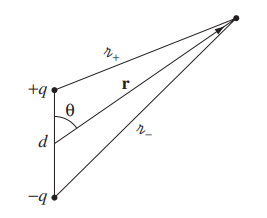
\includegraphics[width=6cm]{Electrodynamics/images/fig3.26.PNG}
\end{center}
Here, note that
\[V(\vec{r})=\frac{q}{4\pi\varepsilon_0}\left(\frac{1}{\scr_+}-\frac{1}{\scr_-}\right).\]
Note that from the law of cosines,
\[\scr_\pm^2=r^2+\left(\frac{d}{2}\right)^2\mp rd\cos\theta=r^2\left(1\mp \frac{d}{r}\cos\theta+\frac{d^2}{4r^2}\right).\]
Since we are interested in the regime $r\gg d$, the third term is negligible, so
\[\frac{1}{\scr_\pm}\approx \frac{1}{r}\left(1\mp \frac{d}{r}\cos\theta\right)^{-1/2}\approx \frac{1}{r}\left(1\pm\frac{d}{2r}\cos\theta\right).\]
Thus,
\[\boxed{V(\vec{r})\approx \frac{qd\cos\theta}{4\pi\varepsilon_0r^2}\qquad (r\gg d)}.\]
\end{proof}

Therefore, the potential of a dipole falls off with $1/r^2$ for large $r$. It makes sense that this falls off more rapidly than a point charge. Further, if we put two opposite dipoles together, we get a \vocab{quadrupole}, and it turns out that this potential falls off with $1/r^3$. We can then place two opposite quadrupoles together to form an \vocab{octopole}, whose potential falls off with $1/r^4$. This is summarized in the following figure:

\begin{center}
    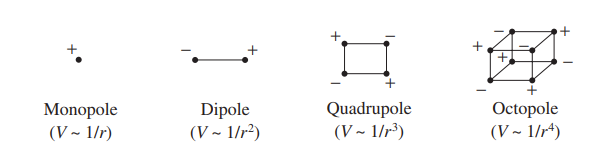
\includegraphics[width=10cm]{Electrodynamics/images/fig3.27.PNG}
\end{center}

Now, let's try to develop this theory for a general charge distribution $\rho$. The necessary variables are defined in the diagram below:

\begin{center}
    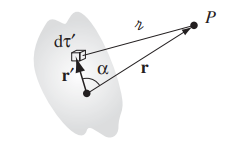
\includegraphics[width=6cm]{Electrodynamics/images/fig3.28.PNG}
\end{center}

Recall that
\[V(\vec{r})=\frac{1}{4\pi\varepsilon_0}\iiint_{\mathbb{R}^3}\frac{\rho(\vec{r'})}{\scr}d\tau'.\]
Using the law of cosines, we have
\[\scr^2=r^2+(r')^2-2rr'\cos\alpha=r^2\left[1+\left(\frac{r'}{r}\right)^2-2\left(\frac{r'}{r}\right)\cos\alpha\right].\]
If we define 
\[\epsilon:=\frac{r'}{r}\left(\frac{r'}{r}-2\cos\alpha\right),\]
then we can Taylor expand
\[\frac{1}{\scr}=\frac{1}{r}(1+\epsilon)^{-1/2}=\frac{1}{r}\left(1-\frac{1}{2}\epsilon+\frac{3}{8}\epsilon^2-\frac{5}{16}\epsilon^3+\cdots\right),\]
and substituting $\epsilon$ gives
\[\frac{1}{\scr}=\frac{1}{r}\left[1+\left(\frac{r'}{r}\right)(\cos\alpha)+\left(\frac{r'}{r}\right)^2\left(\frac{3\cos^2\alpha-1}{2}\right)+\left(\frac{r'}{r}\right)^3\left(\frac{5\cos^3\alpha-3\cos\alpha}{2}\right)\right].\]
Oh, look! The Legendre polynomials have showed up again! This is an alternative way to the Rodrigues' Formula to define the polynomials, where $1/\scr$ is a \textit{generating function} for the Legendre polynomials.
\[\frac{1}{\scr}=\frac{1}{r}\sum_{n=0}^\infty \left(\frac{r'}{r}\right)^nP_n(\cos\alpha).\]
Substituting this back into our formula for the potential gives
\[\boxed{V(\vec{r})=\frac{1}{4\pi\varepsilon_0}\sum_{n=0}^\infty \frac{1}{r^{n+1}}\iiint_{\mathbb{R}^3}(r')^nP_n(\cos\alpha)\rho(\vec{r'})d\tau'}.\]
This is the \vocab{multipole expansion} that we're searching for; it can be written explicitly as
\begin{align*}
V(\vec{r})=\frac{1}{4\pi\varepsilon_0}&\left[\frac{1}{r}\iiint \rho(\vec{r'})d\tau'+\frac{1}{r^2}\iiint r'\cos\alpha \rho(\vec{r'})d\tau'\right.\\
&\left.+\frac{1}{r^3}\iiint(r')^2\left(\frac{3}{2}\cos^2\alpha-\frac{1}{2}\right)\rho(\vec{r'})d\tau'+\cdots\right].
\end{align*}
Note that the first term is precisely $\frac{Q}{4\pi\varepsilon_0r}$ (as the integral of all the volume charge density should be exactly $Q$), what we would expect from a point charge. You can further check that the next term matches with $\frac{qd\cos\theta}{4\pi\varepsilon_0r^2}$ from the dipole moment above. The third is quadrupole, falling off with $1/r^3$; the fourth is octople, falling off with $1/r^4$; and so on.

\begin{remark}
If you're interested in the potential along the $z$-axis (so reorient your coordinate system so that $\vec{r}$ is pointing along the $z$-axis), then $\alpha$ is the usual polar angle $\theta$. 
\end{remark}

This multipole expansion is useful primarily as an approximation scheme, where you add more terms as more precision is needed.

\subsection{The Monopole and Dipole Terms}

At large $r$, the multipole expansion is dominated by the monopole term (as expected):
\[V_{\text{mon}}(\vec{r})=\frac{1}{4\pi\varepsilon_0}\frac{Q}{r},\]
where $Q=\iiint \rho d\tau$ is the total charge of the configuration. Of course, for the particular configuration of a single point charge at the origin, $V_{\text{mon}}$ is the \textit{exact} potential.

If the total charge is zero, this term vanishes, and the multipole expansion is dominated by the dipole term:
\[V_{\text{dip}}(\vec{r})=\frac{1}{4\pi\varepsilon_0}\frac{1}{r^2}\iiint_{\mathbb{R}^3}r'\cos\alpha \rho(\vec{r'})d\tau'.\]
Since $\alpha$ is the angle between $\vec{r}$ and $\vec{r'}$, we can write this more succinctly as
\[V_{\text{dip}}(\vec{r})=\frac{1}{4\pi\varepsilon_0}\frac{1}{r^2}\hat{r}\cdot\iiint_{\mathbb{R}^3}\vec{r'}\rho(\vec{r'})d\tau'.\]

\begin{definition}
The integral here (which luckily no longer depends on $\vec{r}$, since we removed the $\cos\alpha)$, is known as the \vocab{dipole moment} of the distribution:
\[\vec{p}:=\iiint_{\RR^3}\vec{r'}\rho(\vec{r'})d\tau'.\]
\end{definition}

With this definition, the dipole contribution simplifies to
\[V_{\text{dip}}(\vec{r})=\frac{1}{4\pi\varepsilon_0}\frac{\vec{p}\cdot\hat{r}}{r^2}.\]
The dipole moment is determined by the geometry (size, shape, and density) of the charge distribution. For a collection of $n$ point charges $q_i$, the dipole moment is simply
\[\vec{p}=\sum_{i=1}^n q_i\vec{r_i'}.\]
Therefore, for a physical dipole (as in Example \ref{physelecdip}), we have
\[\vec{p}=q\vec{r_+'}-q\vec{r_-'}=q\vec{d},\]
where $\vec{d}$ is the vector of length $d$ from the negative charge to the positive one.

Unlike the monopole, however, this is only the \textit{approximate} potential of the physical dipole, when $r$ is large (or $d$ is small). 

\begin{definition}
A \vocab{perfect dipole} is a physical dipole under the limit $d\to 0$, $q\to \infty$, while keeping the dipole moment $qd=p$ fixed. A perfect dipole's potential is exactly $V_{\text{dip}}$.
\end{definition}

Dipole moments are vectors, and they add like vectors. So given two dipoles with moments $\vec{p}_1$ and $\vec{p}_2$, the total dipole moment is $\vec{p}_1+\vec{p}_2$. Hence, the construction of the quadrupole: by arranging two opposite dipoles next to each other, the dipole moment is zero, so the potential is dominated by the quadrupole term in the multipole expansion.

\subsection{Origin of Coordinates in Multipole Expansion}

A point charge at the origin is a pure monopole. However, if it's off from the origin, it's no longer a pure monopole! For instance, a charge $q$ at $(0,d,0)$ has dipole moment $\vec{p}=qd\hat{y}$.

After all, the exact potential is $\frac{1}{4\pi\varepsilon_0}\frac{q}{\scr}$, not over $\frac{1}{4\pi\varepsilon_0}\frac{q}{r}$ (this is why we need to expand $1/\scr$ as a generating function anyway, to get all the Legendre polynomials/higher order terms).

Note, however, that moving the origin doesn't change the \vocab{monopole moment} $Q$ (or even the monopole term), it's just that the higher poles start to appear. In a similar way, movign the origin affects the dipole moment as well (and the higher pole terms). However, there is a special exception:

\begin{claim}
If the total charge is zero, then the dipole moment is independent of the choice of origin.
\end{claim}

\begin{proof}
If we displace the origin by an amount $\vec{a}$, then the new dipole moment is
\begin{align*}
\vec{p}_{\text{new}}&=\iiint \vec{r'}_{\text{new}}\rho(\vec{r'})d\tau'\\
&=\iiint (\vec{r'}-\vec{a})\rho(\vec{r'})d\tau'\\
&=\iiint \vec{r'}\rho(\vec{r'})d\tau'-\vec{a}\iiint\rho(\vec{r'})d\tau'\\
&=\vec{p}-Q\vec{a}.
\end{align*}
Therefore, if $Q=0$, then $\vec{p}_{\text{new}}=\vec{p}$.
\end{proof}

So if someone asks you for the dipole moment of configuration (a) below, you can confidently say $q\vec{d}$. But if someone asks you for the dipole moment of configuration (b) below, you should respond ``with respect to \textit{what origin}?"

\subsection{The Electric Field of a Dipole}

Let's use the potential to calculate the electric field of a perfect dipole. Change coordinates so that $\vec{p}$ is at the origin and pointing in the $z$ direction, then 
\[V_{\text{dip}}(r,\theta)=\frac{1}{4\pi\varepsilon_0}\frac{\vec{p}\cdot \hat{r}}{r^2}=\frac{p\cos\theta}{4\pi\varepsilon_0r^2}.\]
Now we take the negative gradient of $V$ to get the electric field $\vec{E}$:
\begin{align*}
    E_r&=-\frac{\partial V}{\partial r}=\frac{p\cos\theta}{2\pi\varepsilon_0r^3}\\
    E_\theta&=-\frac{1}{r}\frac{\partial V}{\partial\theta}=\frac{p\sin\theta}{4\pi\varepsilon_0 r^3}\\
    E_\varphi&=-\frac{1}{r\sin\theta}\frac{\partial V}{\partial \varphi}=0
\end{align*}
Hence,
\[\vec{E}_{\text{dip}}(r,\theta)=\frac{p}{4\pi\varepsilon_0r^3}(2\cos\theta \cdot\hat{r}+\sin\theta\cdot\hat{\theta}).\]
This makes explicit reference to a particular coordinate system (spherical), and assumes a particular orientation for $\vec{p}$ (along the $z$-axis). Note that the dipole electric field falls off with the inverse \textit{cube} of $r$ (after all, the monopole field falls of with the inverse \textit{square}). This makes sense since the gradient simply introduces another factor of $1/r$ into the potential drop offs. 

Below is a picture of a pure dipole electric field and a physical dipole electric field. Note how for $r\gg d$, they pretty much agree.

\begin{center}
    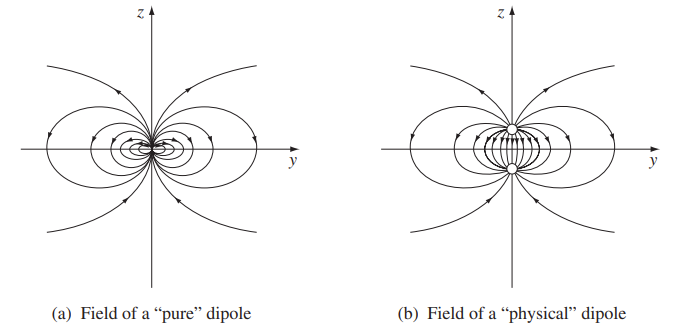
\includegraphics[width=12cm]{Electrodynamics/images/fig3.37.PNG}
\end{center}


\end{document}